% !TeX encoding = UTF-8
% !TeX program = pdflatex
% !TeX spellcheck = en_US

\documentclass[LaM,binding=0.6cm, english]{sapthesis}

\usepackage{microtype}
\usepackage{xcolor}% http://ctan.org/pkg/xcolor
\usepackage{hyperref}
\hypersetup{
  colorlinks=true,
  linkcolor=blue,
  urlcolor=blue
}
\usepackage{glossaries}
\usepackage{graphicx}
\usepackage{subfig}

\hypersetup{pdftitle={Customer Churn Prediction - Energy Provider Case Study},pdfauthor={Vigèr Durand Azimedem Tsafack}}

% Remove in a normal thesis
\usepackage{lipsum}
\usepackage{curve2e}
\definecolor{gray}{gray}{0.4}
\newcommand{\bs}{\textbackslash}

% Commands for the titlepage
\title{Customer Churn Prediction - Energy Provider Case Study}
\author{Vigèr Durand Azimedem Tsafack}
\IDnumber{1792126}
\course[override]{Master’s degree in Data Science}
\courseorganizer{Faculty of Information Engineering, Computer Science and Statistics}
\AcademicYear{2019/2020}
\copyyear{2020}
\advisor{Prof. Anagnostopoulos Aristidis}
\coadvisor[ext]{Andrea Ianni, PhD}
\authoremail{vigerdurand@yahoo.fr}

\examdate{October 30, 2020}
\examiner{Prof. Anagnostopoulos Aristidis}
\examiner{Prof. Name Surname}
\examiner{Dr. Name Surname}
\versiondate{\today}

\begin{document}

\frontmatter

\maketitle

\begin{abstract}

\par The cost of customer acquisition is far greater than cost of customer
retention. This is a known fact across all the industry sectors, making retention a crucial business prototype. Customer churn analysis is one of the most important and common drivers laying behind customer retention. In fact, knowing in advance if a client is about to churn can be a quite valuable information; Particularly in the energy field which is going to be the focus of this work.

\par Energy supply is one of the most competitive industries where large amount of data is usually produced. Therefore, churn prediction in this type of industries is a key tool for customer retention. The present work aims to predict customer churn in energy industry through several data science techniques and methods. The experiment has been held in an Italian energy provider company which provided us with a huge amount of data. we start by explaining some relevant concepts from machine learning and continues to a presentation of related works on the field of customer churn prediction. Then, an empirical study is performed by applying findings from the literature to the data provided by the aforementioned energy provider company. This study can be summarized in two main phases: Data and Modeling. The Data step includes collection, exploration and transformation of data.The Modeling phase refers to the creation and selection of the best machine learning model.

\par Regarding the results, Gradient Boosted Tree Classifier outperformed all the other four models that we tried (Logistic Regression, Decision Tree, Random Forest and XGBoost) with a 27\% and a 54\% of F1 Score on micro and small-medium data clusters respectively. The model evaluation was done by using the following metrics: confusion matrix, Precision, Recall, F1 Score ROC AUC and PR AUC. The study also confirmed that machine learning is a viable tool for predicting customer churn in energy provider companies.

\end{abstract}

\tableofcontents

\printnoidxglossaries

\listoffigures

\listoftables

\mainmatter

\chapter{Introduction}

\par After the industrial revolution and the advent of technical progress, almost all the industrial sectors have become highly competitive in developed countries. The energy sector is certainly not left out since today's costumer won't hesitate to change their energy provider if they do not find what they are looking for or if they get a better offer elsewhere. Knowing that the cost of costumer acquisition is far grater than that of costumer retention, companies try now to focus their attention mostly on retaining existing clients rather searching for new ones.

\par Communications technologies came with great advantages, making our every day live incredibly easy. however, they also represent a big disadvantage for companies since they have empowered the costumers who are no longer stuck with the decisions of a single company. Given that competitors are only one click away, companies must find interesting ways and techniques to examine their clients, understand their behavior and being able to predict if they are possibly going to leave in a close future. One of the tools that is commonly used in customer churn prediction is machine learning.

\par The quantity of companies data is continuously increasing, making the usage of machine learning for customer churn prediction more and more popular in almost every industry. Most machine learning applications work as follow: the data set is split into a test and training data. The training data is then used to train a model that learns from the data. The model is afterwards used to predict the results on yet unseen test data which are then compared to real values. Last but not least, metrics are used to calculate how good the model is doing using real and predicted values.\cite{Geron2017}

\par The aim of this study was to develop a machine learning application namely an efficient and accurate churn prediction model for an energy provider company. In order to settle the context and make you familiar with the research's realm, we start the report by explaining some machine learning theoretical concepts and afterwards we describe the steps that we took in the development process of our churn prediction machine learning model.

\section{Motivation and background}

\par In terms of the economic model, the electricity industry has evolved in time from a vertically integrated state-owned monopoly company (not subjected to the normal rules of competition) to a liberalized market where generators and consumers have the opportunity to freely negotiate the purchase and sale of energy.\cite{Sousa2015} Nowadays, it is crucial for an energy provider to offer a quality service and to invent innovative strategies to increase customer satisfaction in order to retain the maximum number of clients and thus, remain competitive on the market. Machine Learning is a great tool that helps in achieving that goal. Indeed, machine learning based applications turn to be a fruitful avenue of research for data-intensive energy industry.

\par Some of the existing machine learning studies in energy industry include reliability and preventive maintenance, commonly known as failure detection.\cite{Garcia2016} Equipment failure in the energy industry, especially on coal-fired power plants, potentially cause injuries or even the death of workers. Artificial intelligence is helpful in preventing this problem. AI algorithms analyze equipment data and detect failures before they happen to save money, time, and people’s lives. Regarding customer churn predictive analysis which is the goal of this study, after some research, we sadly noticed that it is not extensively studied in energy industry. However, given the actual competitive state of this market, it deserves more attention.

\section{Theoretical framework and focus of the study}

In this study, we mostly focus on exploiting the current state of the literature to empirically build several models for customer churn prediction in energy industry exploiting the provided data. Then suitable metrics are used to evaluate the build models in order to select the best performing one to be used in an Italian energy provider context.

\begin{figure}[!ht]
    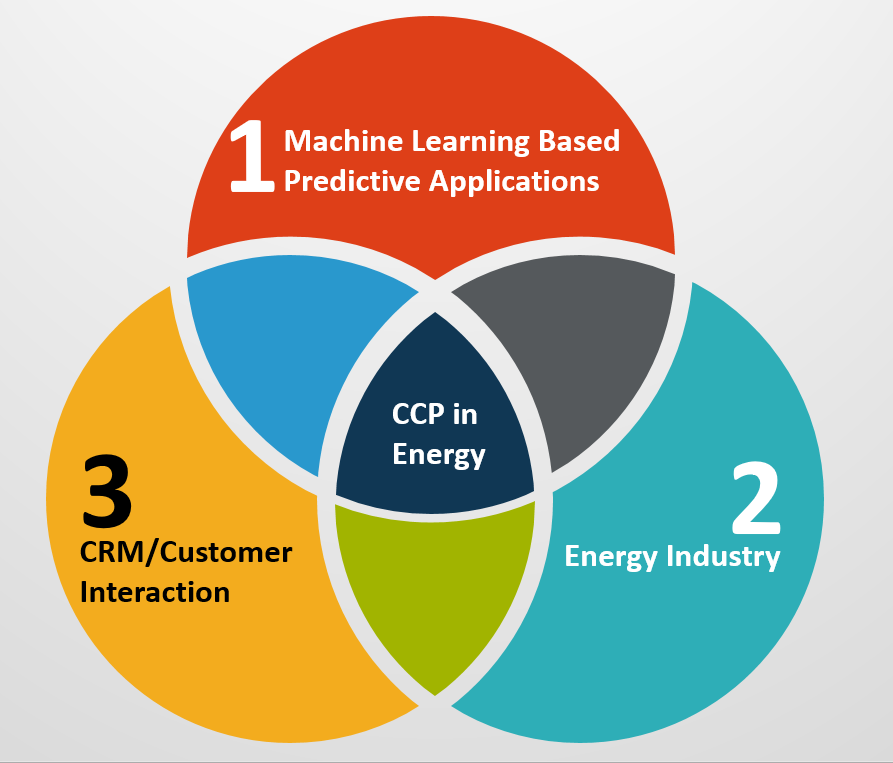
\includegraphics[width=0.5\textwidth]{images/Thesis-Research-Area.png}
    \centering
    \caption{Thesis research area}
    \label{fig:research-area}
\end{figure}

\section{Research questions and objectives}

The primary goal of this thesis is to accurately predict the future churn or status of costumers (stays/churns) for an Italian energy supply company for the next 2 months. Machine learning is the tool that will be used to achieve our goal. Thereby, a theoretical overview of related machine learning concepts is needed in order to create a good model. The obtained models are compared using some metrics an the best performing one is selected to be used in production. Based on these objectives the following research questions are formulated:

\begin{enumerate}
	\item What is the current state of costumer churn prediction in the 			literature?
  	\item What is the current state of costumer churn prediction on the energy supply field?
  	\item Which models can be used to accurately predict costumer churn given customer feature data in energy supply filed?
  	\item How can they be evaluated?
  	\item How different models compare to one another?
\end{enumerate}

\section{Methodology}

The study made in this thesis consisted in three steps. Foremost, some research are formulated based on the desired outcome and the literature. As a first part, we conducted general overview of the machine learning concepts that are necessary to fully understand this thesis. The second part consisted in searching the literature to find related work that were used as inspiration for the last part. Finally, starting from the literature review, we selected some machine learning models and some evaluations metrics to build a churn predictive application.

Data was provided by an Italian energy provider and consisted in real costumer data from January 2019 to March 2020. Unfortunately, for privacy reasons the data cannot be disclosed alongside this thesis.

\section{Structure of the thesis}

The second chapter presents a high level overview of critical methodologies and concepts useful to understand the study performed in this thesis. In the third chapter we perform a review of related existing studies in the field of customer churn prediction. Next, in the fourth chapter an empirical study is conducted to prepare the data and build the churn prediction machine learning model. In chapter five we analyze the model results. Finally in chapter six, we discuss the results, eventual limitations, make the conclusions along with the proposals for future studies on the topic.

\chapter{Machine learning: Some theoretical concepts}

Machine learning is a branch of artificial intelligence that systematically applies algorithms to synthesize the underlying relationships among data and information.\cite{Awad2015} Lately, it has become a common solution to several problems that companies face daily. This chapter presents a high level explanation of some machine learning concepts which the comprehension is necessary to fully understand the experiment performed within the framework of this thesis.

\section{Data collection and preprocessing} \label{data-collection}

Without data, no machine learning project could be made possible. It is therefore crucial to find interesting ways to collect and process the data to make it ready for any machine learning algorithm. Several methods are often used for this purpose. The most relevant for the scope of this thesis will be presented in this section. 

\subsection{ETL}

The acronym ETL stands for Extract, Transform, and Load. ETL tools are pieces of software responsible for the extraction of data from several sources, their cleansing, customization and insertion into a data warehouse.\cite{Vassiliadis2002} These tools are very often used as helper in the process of data collection and preparation for a machine learning application.

\par More explicitly, an ETL tool is three database functions combined into one entity to pull data out of one or multiple database(s) and then place it into another database. The process can be summarized as follows: data is taken (extracted) from a source system, converted(transformed) into a desired format, and finally stored into a data warehouse or other systems.

\subsection{Apache spark} \label{spark}

The quantity of digital data generated in today's companies is continuously increasing thus making their analysis more difficult. To overcome this problem several solutions have been implemented through the years. Google’s MapReduce revolutionized large-scale analysis, enabling the processing of massive data sets on commodity hardware and cloud resources, providing transparent scalability and fault tolerance at the software level.\cite{Capuccini2017} Open source implementations of MapReduce include Apache Hadoop.

\par Industries initially adopted Hadoop because it is a framework based on a simple programming model (MapReduce), it provides a computing solution that is scalable, flexible, fault-tolerent and also cost effective. Apache spark comes into play when the concern is to maintain speed while processing large data sets. It was introduced by Apache Software Foundation aiming to speed up the Hadoop computational process.

\par Apache Spark is designed to accelerate analytics on Hadoop while providing a complete suite of complementary tools that include a fully-featured machine learning library (MLlib), a graph processing engine (GraphX) and stream processing. Spark is natively designed to run in-memory, enabling it to support iterative analysis and more rapid, less expensive data crunching. Spark runs programs in memory up to 100 times faster than Hadoop MapReduce and up to 10 times faster on disk. Spark's speed and efficiency are some of the the key reasons behind it's popularity. 

\subsection{Dealing with missing data} \label{missing-data}

Data is the hub of every machine learning project. As a matter of fact without a good and clean data set, useful results cannot be obtained from the data science process. Missing data is a major problem that statisticians and data scientists face quite often.

\par Dealing with missing data is absolutely necessary because most statistical models operate only on complete observations of predictor and target variables. Different methods can be adopted to deal with missing data. Incomplete observations can be deleted or missing values can be replaced by an estimated value based on other information available. This process is called missing data imputation.\cite{Salgado2016} To handle missing data, three main steps are generally followed: (i) finding the reasons for missing data; (ii) analyzing the proportions of missing data by feature and finally; (iii) choosing the best imputation method. Analyzing the cause of missing data is very important since it plays a major role in the choice of the imputation technique to be used.

%\par In terms of source of "missingness", several cases are possible: (i) the value is missing because it was forgotten or lost (Missing Completely at Random); (ii) the value is missing because it was not applicable to the instance (Missing at Random); (iii) the value is missing because it is of no interest to the instance (Missing Not at Random).\cite{Salgado2016} Let's rewrite this adapting it to the energy supply context: (i) the variable is correctly calculated but for some reason that cannot be identified, the values are not written in the database, eg. failure of ETL process, communication errors while writing the values in the database, values accidentally deleted, and others; (ii) The variable is not calculated during a certain amount of time due to an identifiable reason, for example the system is down for maintenance reasons; (iii) the variable is not calculated because it not relevant for that particular type of client, for instance the number of family members is not relevant if the client is a company.

\subsection{Dealing with imbalance data} \label{imbalance_data}

Imbalanced training data set means that one class is represented by a large number of observations (majority class) while the other is underrepresented, namely represented by only a few number of observations (minority class). This is a typical issue that is observed with every churn prediction problem. It may produce an importance deterioration of the classification accuracy, leading for example to all the observations being predicted as part of the majority class. Several techniques are usually adopted to handle the imbalance situation. The two most common are the under sampling and over sampling approaches.\cite{Barandela2004}

\subsection{One-hot encoding} \label{one-hot_encoding}

Most machine learning and deep learning models require all input and output variables to be numeric. This means that if the data set contains categorical data, that data must be converted into numerical form before fitting it to a machine learning model. One-hot encoding method is one of the most commonly used strategies to convert data from categorical to numerical form. This technique requires very little work. With this method, categorical variables are converted into several binary columns.

\begin{figure}[!ht]
    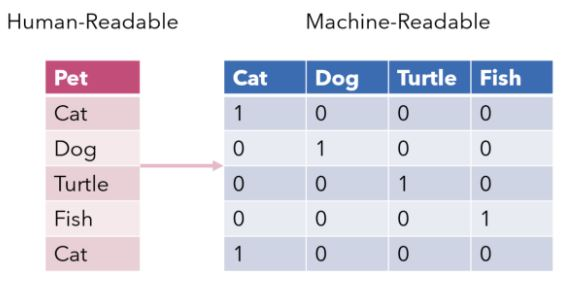
\includegraphics[width=0.5\textwidth]{images/One-hot_encoding.jpg}
    \centering
    \caption{One-hot encoding method}
    \label{fig:one-hot-encoding}
\end{figure}

\par One clear disadvantage of this method is the fact that the distance between one-hot encoded vectors does not carry much information. Another major disadvantage is that it aggressively consumes storage resources.\cite{Hancock2020}

\subsection{Ordinal encoding} \label{ordinal_encoding}

Another important and widely used method to convert features from categorical form to numerical is ordinal encoding. this method is generally used when the variable to be converted is ordinal, namely when the variable comprises a finite set of discrete values with a ranked ordering between values. For instance, if the possible values of the variable are \textit{first}, \textit{second} and \textit{third}, integers \textit{1}, \textit{2} and \textit{3} can be used to encode the variable. 

\par An advantage of this method is that since the integer values have a natural order relationship between each other, machine learning algorithms may be able to understand and use this relationship. A clear disadvantage is that it cannot be used to encode every type of categorical feature since it is adapted only for features presenting a natural ordinal relationship among the possible values.

\subsection{Categorical embeddings} \label{categorical_embeddings}

The standard in natural language processing (NLP) is to encode the input such as words into continuous vector representation which are called embeddings.\cite{Almeida2019} Embeddings are a solution to dealing with categorical variables while avoiding a lot of the pitfalls of one-hot encoding. Recently, there has
been some interest in learning embeddings \cite{Hannes}, \cite{Berkhahn2016}, \cite{Russac2018} for general
categorical variables instead of using the standard encoding
techniques. Formally speaking, an embedding is a mapping of a categorical variable into an n-dimensional vector.

This provides us with 2 advantages. First, we limit the number of columns we need per category. Second, embeddings by nature intrinsically group similar categories together.

\subsection{Feature selection} \label{feature_selection}

Feature selection is the process of manually or automatically selecting the features contributing the most to the prediction of the target variable. As the number of variables and data has increased due to more advanced data gathering, it is essential to include only the most critical and useful variables for the model one is building. Feature selection have three main objectives: (i) Allowing the model to achieve better predictive performance; (ii) getting faster and more efficient predictions; (iii) Allowing to get a more understandable and interpretable model. Adding unnecessary variables to the model also adds unnecessary complexity and can lead to overfitting, while missing essential variables lead to the reduction of the predictive performance. Feature selection methods can be divided into three main category: \textit{Filter} methods, \textit{Wrapper} methods and \textit{embedded} methods.\cite{duboue2020}

\par In \textit{Filter} methods, a relevance criteria is initially decided. Subsequently, the features are ranked based on the previously decided criteria. A threshold is set to select the highest-ranking features. Some commonly used metrics are the following: (i) variance which is used to remove constant features; (ii) chi-square which is a statistical test that is used to verify the dependency of two variables; (iii) correlation coefficients that can be used to remove duplicated variables. 

\par \textit{Wrapper} method feature selection process is based on a specific machine learning algorithm that we wish to fit on a given data set. A greedy search approach is used by evaluating all the possible combinations of features against the evaluation criterion. even if this method is effective, it is also computationally expensive.

\par In \textit{embedded} methods, the feature selection process is completed within the machine learning algorithm itself. In other words, the feature selection process is performed during the model training.

\par Another method which is quite common is to use principal component analysis (PCA), which is a linear extraction method that transforms the data into a low-dimensional subspace. The idea is to retain most of the information but reduce the features into a smaller vector.\cite{Jolliffe2016}

\section{Machine learning models}

Several machine learning algorithms have been used in this thesis. In this section we provide a theoretical explanation for all of them.

\subsection{Logistic regression} \label{lr_model}

Logistic regression is one of the most common machine learning algorithms. It is generally used as a baseline model when the problem to be solved is a classification problem. This model is particularly appropriate when the dependent variable is dichotomous (binary).\cite{Sahar2018} The name logistic regression is derived from the function used at the core of the method to transform the linear predictions, the logistic function. The logistic function which is also known as sigmoid function is a very popular function that machine learning borrowed from the statistical field. It is an S-shaped curve that can take any real-valued number and map it into a value between 0 and 1, but never exactly at those limits. The logistic function can be mathematically expressed as shown in equation \ref{eqn:logistic-function}.

\begin{equation}
\label{eqn:logistic-function}
logit(x) = \frac{1}{1 + e^{-x}} = \frac{e^x}{1 + e^x}
\end{equation}

\par Every linear methods try to fit a curve between data points. While \textit{linear regression} uses the least-squares method to measure the error namely the distance between the data points and the line, logistic regression in contrast uses maximum likelihood in its fitting process. Maximum likelihood tries to maximize the probability of obtaining the observed data set using the likelihood function. The chosen maximum likelihood estimators are those maximizing the likelihood function and agreeing the most with the data. Equation \ref{eqn:logistic-regression} shows a mathematical representation of logistic regression.

\begin{equation}
\label{eqn:logistic-regression}
logit(\pi(x)) = \beta_0 + \beta_1x_1 + ... + \beta_nx_n \Longleftrightarrow \pi(x) = \frac{e^{\beta_0 + \beta_1x_1 + ... + \beta_nx_n}}{1 + e^{\beta_0 + \beta_1x_1 + ... + \beta_nx_n}}
\end{equation}

where \(\pi(x)\) is the probability of the predicted event, \(\beta_i\) is the regression coefficient for each explanatory variable \(x_i\). The probability of belonging to the predicted class is obtained by solving \(\pi(x)\) from the equation.\cite{Hosmer2000}

\subsection{Decision tree classifier} \label{dt_model}

Another commonly used model for solving classification problems in machine learning is decision tree. A decision tree is simply a supervised machine learning algorithm where the data is continuously split according to a certain parameter. It is a very simple model. Given several features, the decision begins with one of these features; if that is not enough, we use another one, and so on. 

\par It is widely known and used in many companies to aid the decision making process and risk analysis. It was widely used from the 1960s to the 1980s for building expert systems. The rules were entered manually, that is why this model lost its popularity after the 1980s. The advent of mathematical methods to build decision trees brought this model back to the battle of automatic matching algorithms. The following is the general algorithm for creating a decision tree:

\begin{enumerate}
	\item Determine the best feature from the training data set.
  	\item Divide the training data into subsets containing the possible values of the best feature.
  	\item Recursively generate new decision trees using the created data subsets.
  	\item We stop when we can no longer classify the data.
\end{enumerate}

There are different types of decision trees, among which CART, C4.5, CHAID, QUEST, and more...\cite{Song2015} CART which stands for classification and regression trees is the most commonly used by the models that were considered in this study. Figure \ref{fig:decision-tree}, displays a simple binary decision tree.

\begin{figure}[!ht]
    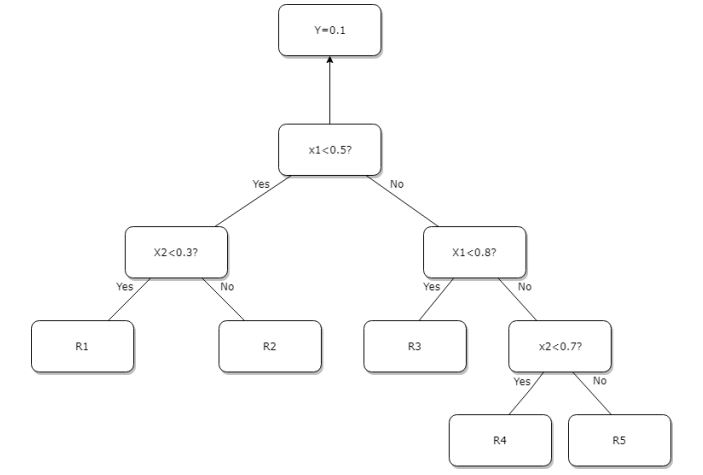
\includegraphics[width=0.8\textwidth]{images/Simple_Decision_Tree.jpg}
    \centering
    \caption{A decision tree example based on binary feature Y \cite{Song2015}}
    \label{fig:decision-tree}
\end{figure}

\par among the advantages of decision trees, we can enumerate the following: (i) they are easy to understand and interpret since the tree can be visualized and the obtained results explained easily; (ii) they can work on data with little preparation, for instance they don't need data standardization; (iii) they accept both numeric and nominal data while other learning algorithms specialize in a single type of data.

\par On the other hand, decision trees present several downsides: (i) they can be complex, they don't generalize well (overfitting), This can be adjusted by tuning the maximum depth of the tree or the minimum number of samples in the leaves; (ii) they may be unstable due to variations in the data; (iii) some concepts can be difficult to learn using decision trees since they are not easy to express, \textit{XOR} is a good example; (iv) they can be biased towards the ruling class, thus the data has to be balanced before training the system. (v) hitting the optimal decision tree is not guaranteed.

\subsection{Random forest classifier} \label{rf_model}

This powerful machine learning algorithm makes it possible to make predictions based on the aggregation of several decision trees. The method uses binary decision trees, in particular CART trees proposed by Breiman et al. (1984). The general idea behind the method is the following: instead of trying to get an optimized method all at once, we generate several predictors before putting together their different predictions.

\par Random forests are an improvement of bagging for CART decision trees with the aim of making the trees used more independent (less correlated). Some characteristics of this method are that (i) They give good results especially  with large data sets; (ii) They are very easy to implement; (iii) They have few parameters.\cite{Fang2016} The general steps for implementing this model are the following:

\begin{enumerate}
	\item We draw at random from the training set \(B\) samples with replacement \(z_i, i = 1, ..., B\) each sample having \(n\) data points.
  	\item For each sample \(i\) we build a CART tree \(G_i(x)\) according to a slightly modified algorithm: each time a node has to be cut (“split” step) we randomly select a part of the attributes (\(q\) among the \(p\) attributes) and we choose the best division in this subset.
  	\item For classification problems which are of interest in this study, aggregation by vote is used: \(G(x) = Majority vote(G_i(x), ..., G_B(x))\).
\end{enumerate}

\subsection{Boosting: Gradient-boosted tree, XGBoost} \label{boosting_model}

Boosting is another type of ensemble method just like random forests. The principle of boosting is to combine the outputs of several weak classifiers to obtain a stronger result (strong classifier). The weak classifier must have a basic behavior being a little better than the random one: error rate less than 0.5 for a binary classification. Each weak classifier is weighted by the quality of its classification: the better it classifies, the more important it will be. Misclassified examples will have greater weights (they are said to be boosted) towards the weak learner in the next round so that it addresses the gap.\cite{Freund}

\par Gradient boosting is a particular boosting technique which is  mainly used with decision trees. The main idea here is again to aggregate several classifiers together but by creating them iteratively. These “mini-classifiers” are generally simple and parameterized functions, most often decision trees in which each parameter is the criterion for splitting the branches. The final super-classifier is a weighting of these mini-classifiers. One approach to build this super-classifier is to:

\begin{enumerate}
	\item Randomly set the weighting (weights \(w_i\) of the mini-classifiers to form the initial super-classifier.
  	\item Calculate the error induced by this super-classifier, and find the mini-classifier that comes closest to this error.
  	\item Subtract the mini-classifier from the super-classifier while optimizing its weight with respect to a loss function.
  	\item Repeat the process iteratively.
\end{enumerate}

Some of the most common boosting ensemble model implementations are \textit{Gradient-boosted tree} and \textit{XGBoost}. These two algorithms are indeed going to be used in this study.


\section{Evaluation metrics}

The choice of the best performing model is a critical task in machine learning since choosing the wrong model makes all the hard work performed useless. In this section, we give a theoretical explanation of the evaluation metrics used in this thesis.

\subsection{Confusion matrix}

A Confusion Matrix or contingency table is a tool for measuring the performance of a machine learning model by checking in particular how often its predictions are accurate compared to reality in classification problems. More specifically, it is a summary of the results of predictions about a classification problem. Correct and incorrect predictions are highlighted and broken down by class. The results are thus compared with the actual values.

\par This matrix helps to understand how the classification model is confused when making predictions. This not only allows you to know what mistakes were made, but above all the type of mistakes made. Users can analyze them to determine which results indicate how errors are made. To illustrate the idea, we can think of the problem as a binary classification problem where the instance either is classified correctly or is not. In this case, there are four possibilities:

\begin{itemize}
	\item True Positives (TP): cases where the prediction is positive, and where the real value is indeed positive.
  	\item True Negatives (TN): cases where the prediction is negative, and where the real value is indeed negative.
  	\item False Positives (FP): cases where the prediction is positive, but the true value is negative.
  	\item False Negatives (FN): cases where the prediction is negative, but the actual value is positive.
\end{itemize}

\par Several other metrics (\textit{accuracy}, \textit{precision}, \textit{recall}, \textit{f-Score}, ...) can be calculated directly from the confusion matrix. and some of them will be covered subsequently. Figure \ref{fig:confusion-matrix} shows a simple illustration of a confusion matrix configuration.

\begin{figure}[!ht]
    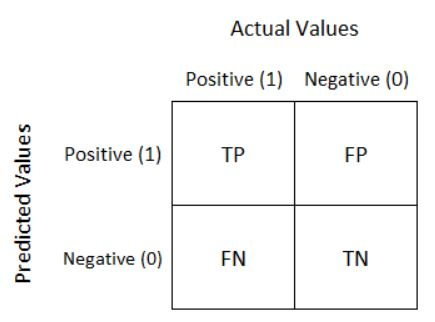
\includegraphics[width=0.5\textwidth]{images/confusion-matrix-exemple.jpg}
    \centering
    \caption{A confusion matrix example}
    \label{fig:confusion-matrix}
\end{figure}

\subsection{Precision, Recall, F-Measure}

Precision, recall and F-Measure are by far the most commonly used evaluation metrics when we want to deal with classification problems. Indeed, in many machine learning problems the performance of algorithms is evaluated using precision and recall measurements.\cite{Sokolova2006} However, these two measures can have a very different importance depending on the
context. That's why data scientist more often prefer an evaluation metric that will combine these two measures equally important one as the other. The most common among those combination metric is called F-Measure (a.k.a f1 score).\cite{Albatineh2011}

\textbf{Precision} can be defined in machine learning as the conditional probability that a randomly chosen example is correctly classified by the system. This is the ratio between the number of true positive predictions (TP) and the number of positive predictions (TP + FP). In our context, it measures the quality of the predictions, that is, the degree to which customers marked as being churning really are. The \textbf{recall} measures the "width of learning" and represents the ratio of the number of true positive predictions to the total number of real positive examples. It measures the percentage of churning clients that was identified by the model, namely the model effectiveness. The break-even point is reached when precision and recall are equal.\cite{Namburu2005} The expression to calculate both precision an recall can be seen in Equation \ref{eqn:precision-recall}.

\begin{equation}
\label{eqn:precision-recall}
Recall = \frac{TP}{TP+FN} \qquad Precision = \frac{TP}{TP + FP}
\end{equation}

\par The \textbf{F-measure}, also called Dice index, can be defined as the harmonic mean of precision and recall. This measurement can be seen as a trade off between precision and recall. Equation \ref{eqn:f-measure} shows the mathematical formula for this metric.

\begin{equation}
\label{eqn:f-measure}
F-measure = \frac{2 * precision * recall}{precision + recall}
\end{equation}

A value close to 1 indicates that the classification is of very good quality.

\subsection{Area under the curve (ROC AUC, PR AUC)}

Other two interesting evaluation metrics in machine learning are the areas under the ROC and PR curves.\cite{Fogarty2005} these two measurements are popular because they are suitable when the data set used to build the model is unbalanced. Indeed, they are going to be perfect for our case, especially area under the PR curve since we wish to have a good recall while keeping the precision reasonably high.

A receiver operating characteristic (ROC) curve is a graph representing the performance of a classification model for all classification thresholds. This curve plots the rate of true positives as a function of the rate of false positives. The true positive rate (TPR) is the equivalent of the recall. It is therefore defined as already shown in equation \ref{eqn:precision-recall}, whereas the false positive rate (FPR) can be expressed as shown in equation \ref{eqn:fpr}. Similarly, A Precision-Recall (PR) curve is another graph that can be used to evaluate a classification model over multiple classification thresholds. This other curve plots the precision as a function of the recall. In summary, These two curves are quite interesting because they can be used to identify the best threshold (namely the one yielding the best performance) for a particular classifier.

The closer to 1 are the areas under the ROC and the PR curves, the better the classifier is likely to perform. Figures \ref{fig:roc_curve_interpretation} and \ref{fig:pr_curve_interpretation} help understanding how the areas under the curves should be interpreted.

\begin{equation}
\label{eqn:fpr}
FPR = \frac{FP}{FP + TN}
\end{equation}

\begin{figure}[!ht]
  \centering
  \subfloat[ROC curve.]{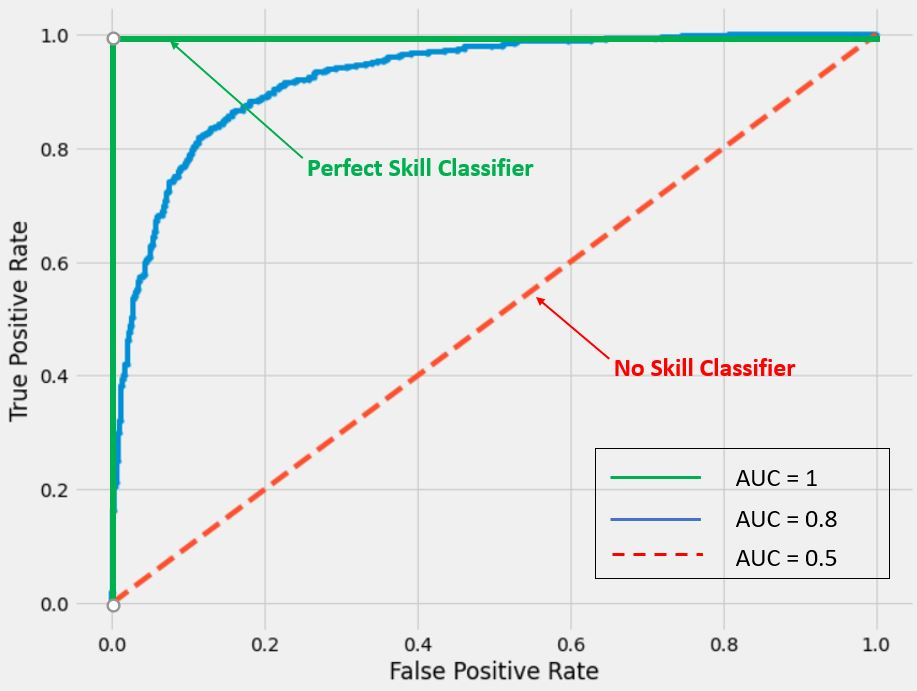
\includegraphics[width=0.5\textwidth]{images/roc_curve_interpretation.jpg}\label{fig:roc_curve_interpretation}}
  \hfill
  \subfloat[PR curve.]{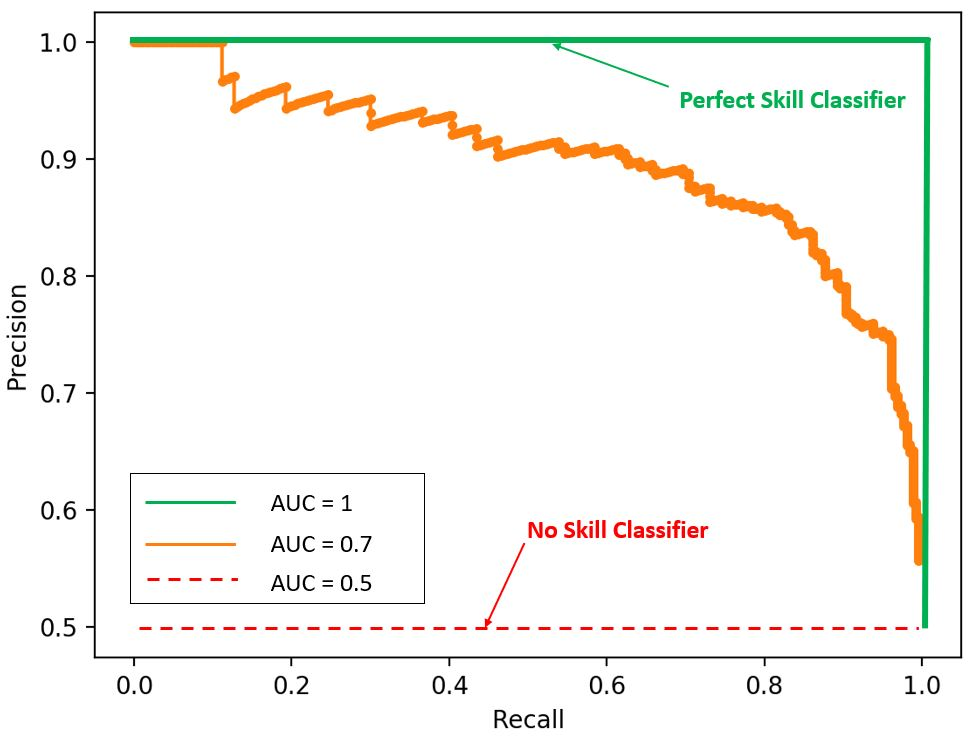
\includegraphics[width=0.5\textwidth]{images/pr_curve_interpretation.jpg}\label{fig:pr_curve_interpretation}}
  \caption{ROC and PR curves interpretation}
\end{figure}

\chapter{Related work}

The word "churn" - which originated from the contraction between the words \textit{change} and \textit{turn} - describes the phenomenon of losing a customer. It is measured by the rate of churn which is an important indicator for organizations. This churn rate represents the percentage of lost customers over a given period compared to the
total number of clients at the beginning of the same period. Reduce this rate is thus one of the most important concerns of every modern company. This study is clearly not the first of his kind. Multiple studies in the field of churn prediction/reduction have been performed, this chapter brings to light some of them reviewing both the techniques and the data sources used.

\section{Review: Techniques and Data}

The goal of the studies on the churn phenomenon is to detect individuals who intend to leave the organization in order to improve decision making and initiate retention actions. It is often analyzed using predictive techniques similar to datamining. Some methods are commonly used for churn prediction, such as logistic regression models (\cite{Nie2009}, \cite{Dahiya2015}, \cite{Yabas2013}, \cite{Rehman2013}), decision tree models (\cite{Dahiya2015}, \cite{Yabas2013}, \cite{Yabas2013}, \cite{Rehman2013}), support vector machines (\cite{Toderean2016}), random forests (\cite{Yabas2013}), neural networks (\cite{Rehman2013}).

\par in \cite{Toderean2016}, a data mining method is used to predict the customer churn in mobile telecommunication industry using call detail records data set that consists of 3333 customers with 21 attributes each and a churn dependent variable with two classes Yes/No. Few attributes include the information about their corresponding inbound/outbound SMS count and voice mail. In this study, a principal component analysis was used in order to reduce the data dimensionality and deal with multicolinearity. the modeling phase was done using three machine learning model, namely support vector machines, neural networks and Baysian networks. In the evaluation phase of this study, confusion matrix and ROC curve were used as evaluation metrics.

\par Another interesting churn prediction study is the performed in \cite{Dahiya2015}. in this study, a software called \textit{WEKA} is used to develop a churn prediction model. Each customer was classified as a potential churner or non-churner. The framework discussed was based on Knowledge Discovery Data process. Three different data sets, small, medium and large with varying attributes were considered. The performance of decision trees and logistic regression models are compared by calculating the accuracy and error rate.

\par Paper \cite{Yabas2013} presents a study on subscriber churn analysis and prediction for mobile and wireless service providers. A real and complied data set by Orange Telecom, 2009 was used. Main emphasis was laid on ensemble methods that encompass single methods to improve the solution to churn prediction problem. These results were compared with that of classic methods, namely logistic regression, decision trees and random forests; the evaluation metric used was ROC score.

\par Paper \cite{Nie2009} proposes a framework of the whole process of churn prediction of credit card holders. The machine learning model used in this study is logistic regression applied on the data of more than 5000 credit card holders provided by a major China commercial bank. Accuracy and ROC curve are used to evaluate the obtained model.

\section{Summary}

Several studies on churn prediction attempt to find the most efficient data mining technique in terms of minimizing the error rate and prediction accuracy. From the researches that have been performed,it turns out that logistic regression random forest and decision trees are the most widely used techniques for churn prediction. In addition, the general remark resulting from this non-exhaustive summary is that there is no standard technique for solving the problem of churn prediction because the quality of the results obtained is closely related to the nature of the data used, their volume and quality, the number and relevance of indicators taken into consideration, the size of the learning sample, and finally the definition of the target variable. Without forgetting the confidential aspect of the data which does not allow the dissemination of the strategic results of the organization, especially in a competitive sector such as energy supply. Figure \ref{fig:studies-summary} synthesizes the articles that we presented in the previous section.

\begin{figure}[!ht]
    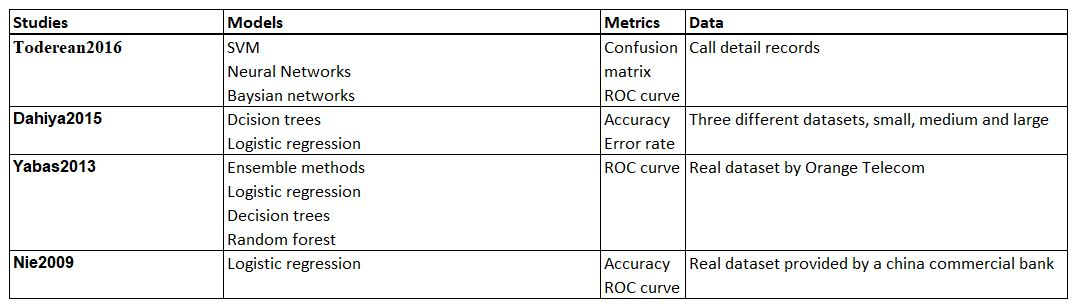
\includegraphics[width=0.95\textwidth]{images/studies_summary.jpg}
    \centering
    \caption{Related works summary}
    \label{fig:studies-summary}
\end{figure}

\chapter{Energy provider case study: churn prediction machine learning model}

According to the US Energy Information Administration (\href{https://www.eia.gov/}{EIA}), Italy is the fourth-largest energy consumer in Europe; the energy market is thereby highly competitive. At this point, the only way for companies of this sector to secure a good market share is to develop various strategies in order not to lose their clients. One of those ways is churn prediction which is the main goal of this work consisting of an experiment that has been performed to meet the needs of one of the largest energy distribution companies in Italy. Machine learning was chosen as the main tool among others to be used in this work. The current chapter describes the development process of our solution.
 
\section{Tools and libraries}

This section presents two important tools that played an essential role in the realization of this work.

\subsection{Python}

Python was chosen as the programming language to be used in this work. It is the most widely used open source programming language. it is also the best language for performing data analysis tasks because it allows developers to focus on what they do rather than how they do it. It freed developers from the form constraints that occupied their time with older languages. Thus, developing code with Python is faster than with other languages. Furthermore, python includes a very large number of libraries that make the data scientist's job easier. \textit{Pyspark} is one of those.

\subsection{Apache Spark}

Apache Spark is a fast data processing engine dedicated to big data. It allows processing of large volumes of data in a distributed manner (cluster computing). It is very popular for a few years now, this Framework is on the way to replace \textit{Hadoop}. Its main advantages are its speed, ease of use, and versatility. Section \ref{spark} presents more details about spark. The native language of apache spark is \textit{scala}; however, in this work we used a version of spark especially designed for python which is called \textit{pyspark}. This version helps to take advantage of the velocity of spark while keeping the simplicity provided by python.

\section{Data collection}

Without Data, no data science study can be performed. This is the reason why we had to implement various logics to gather customer data all over the company.

\subsection{Data collection: ETL}

Apache spark engine works with full potential within a cluster; That is why is was necessary to transfer the data from all over the company to a \textit{cloudera} cluster. Another important goal of this step was to gather all the needed customer data at one place in order to process it more efficiently taking advantage of the processing speed of spark. Multiple ETL processes have been developed to transfer clients data from multiple scopes to the cloudera cluster. Some of the scopes from which data was pulled are billing, marketing, customer relationship management (CRM), contacts, pricing, complaints management, etc. Figure \ref{fig:data-collection} schematically shows the implemented workflow. 

\begin{figure}[!ht]
    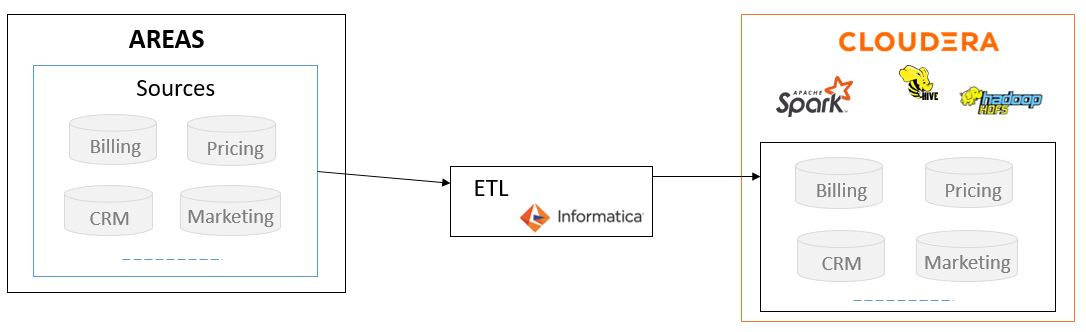
\includegraphics[width=0.95\textwidth]{images/data_collection.jpg}
    \centering
    \caption{Data collection}
    \label{fig:data-collection}
\end{figure}

\subsection{Feature creation} \label{feature-creation}

After collecting the customer data and loading it into the cloudera cluster, we started working effectively on the churn prediction model which is the scope of this thesis. The first step in this process was feature creation which is essential for every data science project. In this step, we merged the gathered data to obtain the data set to be used in the modeling phase. This phase was performed writing a python code that implemented the following steps: (i) Initial time-stamps \textit{t0's} was chosen (15 time-stamps, from 01 January 2019 up to 01 March 2020). (ii) At each instant \textit{t0}, a picture of the data was taken by computing some customer related metrics that were thought to be related to the churn phenomenon (Number of inbound calls during the last month, If the client payed late in the last month, etc.); 767 features have been generated. See figure \ref{fig:feature-creation} for a schematical representation of this phase.

\begin{figure}[!ht]
    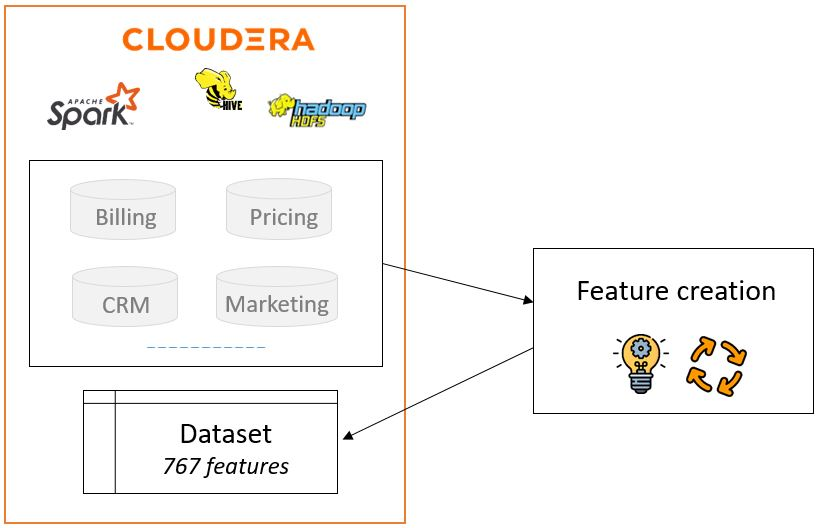
\includegraphics[width=0.95\textwidth]{images/feature_creation.jpg}
    \centering
    \caption{Feature creation}
    \label{fig:feature-creation}
\end{figure}

\section{Data description and understanding}

The task we performed in the current study was that of predicting the churn probability of the business clients of an Italian big energy provider company. As required by the company, the data set has been divided in two distinct groups based on their sizes. The first group consisted in all the clients holding businesses of limited size (\textit{micro}); While the second group consisted in all the clients holding small and medium businesses (\textit{small} and \textit{medium}).

The data set of micro clients consisted of 20.223.914,0 records while the data set of small and medium clients had 5.264.625,0 records. both data sets were made up of 767 columns with 1 boolean target variable indicating weather the client churned two months after \textit{t0} or not. \textit{t0} being the feature creation data already discussed in section \ref{feature-creation}. As shown in figures \ref{fig:target-variable-distribution-micro} and \ref{fig:target-variable-distribution-small-medium}, both data sets were highly unbalanced with the \textit{staying} class highly over represented.

\begin{figure}[!ht]
  \centering
  \subfloat[Micro.]{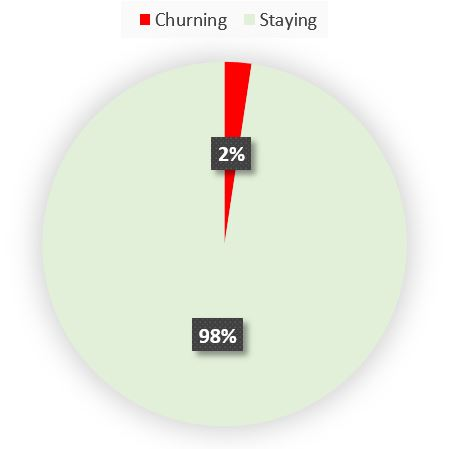
\includegraphics[width=0.45\textwidth]{images/target-variable-distribution-micro.jpg}\label{fig:target-variable-distribution-micro}}
  \hfill
  \subfloat[Small and Medium.]{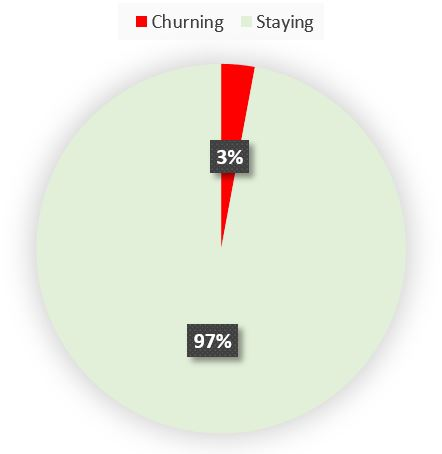
\includegraphics[width=0.45\textwidth]{images/target-variable-distribution-small-medium.jpg}\label{fig:target-variable-distribution-small-medium}}
  \caption{Target variable distribution}
\end{figure}

\section{Data preprocessing and feature selection}

Before applying any machine learning algorithm, some preprocessing steps are usually performed on data in order to clean it and put it in the appropriate form to be best exploited by the algorithm. This section presents the description of the preprocessing/cleaning operations that we performed in this study.

\subsection{Handling missing data}

As previously discussed in section \ref{missing-data}, the first thing to do while handling missing data is to discover the reason why data is missing. This is exactly what we did while dealing with 111 over 767 features that contained missing values for both \textit{micro} and \textit{small-medium} data sets. Some features were removed because they had a high proportion of missing data.

The two principal reasons of data missingness in this study were the following: (i) Missing data caused by software bugs. Indeed, some bugs were present in the ETL processes of the various areas and were propagated into our data sets. In this case, the missing values were imputed by the neutral value already part of the values list. \textbf{e.g.} For the feature \textit{"last bill cluster"} missing values were imputed by \textit{"other"}. (ii) Missing data caused by the fact that the feature were not applicable to the corresponding observation. In this case the missing values were imputed using a new value not yet part of the values list. \textbf{e.g.} For the feature \textit{"number of days since last inbound contact"} missing values were imputed by \textit{-1} which was not yet part of the values list.

\subsection{Dealing with categorical features}

Generally speaking, a data set (textual data and images are excluded) has two types of features: quantitative and qualitative features. A quantitative feature admits numerical, continuous or discrete values. Since these variables are numeric, their processing by machine learning algorithms is simpler, that is, they can be used directly without requiring a prior transformation. A qualitative variable on the other hand takes values called categories, modalities or levels which do not have a quantitative meaning. The presence of these variables in the data generally complicates learning. This is because most machine learning algorithms take numeric values as input.

To deal with this issue, multiple methods already discussed in section \ref{data-collection} have been applied.

\subsubsection{One-hot encoding}

As explained in section \ref{one-hot_encoding}, this method is one of the most commonly used. 12 features have been converted using this method. we chose this method because of the small amount of distinct values in these 12 features, limiting the number of new generated features. This method was applied when the feature was thought not to be further exploitable. The following are some of the 12 features transformed using one-hot encoding: \textit{usage type}, \textit{payment type}, \textit{selling company}, \textit{land type}, etc. 

\subsubsection{Boolean encoding}

As suggested by the name, the features on which this method has been applied were those presenting boolean properties. Namely, having two possible values - one representing \textit{false} and the other \textit{true} - that can respectively be replaced by \textit{0} or \textit{1}. 3 features were affected by this method: (i) \textit{resident}, indicating whether or not the client is resident in his billing municipality; (ii) \textit{win back}, indicating whether or not a win back action has been initiated on the client; (iii) \textit{web bill}, indicating whether or not the client activated the web bill.

\subsubsection{Ordinal encoding}

This is another major encoding method as discussed in \ref{ordinal_encoding}. 9 features have been converted using this method (eg. \textit{consumption quantity cluster}, \textit{customer seniority cluster}, \textit{client size}, etc.). This approach was adopted in order to deal with features presenting a possibility to naturally order their different values.

\subsubsection{Categorical embeddings}

This method was borrowed from the NLP world because of its capability to embed in a M dimensional vector information about the lexical meaning of words learned from various contexts. The context in this case was built selecting several features to form \textit{sentences}. The \textbf{Word2Vec} algorithm was then used to learn 8 dimensional embeddings of each word from the created corpus. Figure \ref{fig:categorical-embeddings} illustrates the process by showing the plot of the embedings of the feature \textit{acquisition channel}.

\begin{figure}[!ht]
    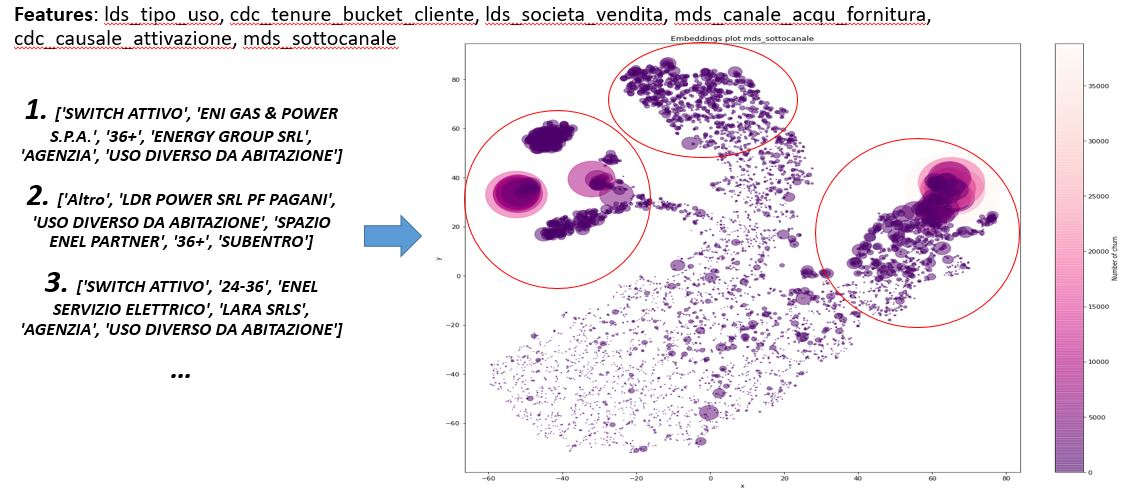
\includegraphics[width=0.95\textwidth]{images/categorical_embeddings.jpg}
    \centering
    \caption{Categorical embeddings: \textit{acquisition channel}}
    \label{fig:categorical-embeddings}
\end{figure}

\subsection{Train-Test split}

This is a traditional step of most machine learning problems. In this step the data set has been divided in two blocs, the training set and the test set. We applied this to both \textit{micro} and \textit{small-medium} data sets. 80\% of the data was used as training data while 20 \% as testing data.

The split operation was performed implementing a stratified random sampling operation with the help of the \textit{pyspark} library in order to maintain the natural distribution of the data. The sampling operation was performed grouping the data by \textit{year}, \textit{month} and \textit{churn}. 80\% of data was selected from each sub group as training data while 20\% as test data. This technique was also used in this study to perform undersampling to deal with the imbalance situation.

\subsection{Imbalanced data}

As already mentioned in \ref{imbalance_data}, having an imbalance data set is a major issue in several machine learning problems. Churn prediction is certainly not an exception. As shown in figures \ref{fig:target-variable-distribution-micro} and \ref{fig:target-variable-distribution-small-medium}, the data sets we worked with were highly unbalanced as we could expect since in a normal situation, the number of churning clients should be typically low. Figures \ref{fig:distribution-over-months-micro} and \ref{fig:distribution-over-months-small-medium} display the quantity distribution of our two training sets over the months for both churning and staying clients. We can clearly see on this figures, the big difference in quantity between the two distributions.

\begin{figure}[!ht]
  \centering
  \subfloat[Micro.]{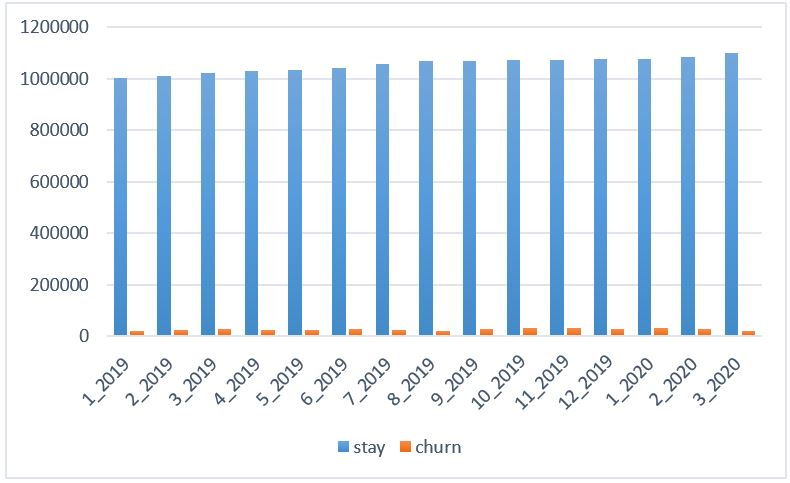
\includegraphics[width=0.50\textwidth]{images/distribution-over-months-micro.jpg}\label{fig:distribution-over-months-micro}}
  \hfill
  \subfloat[Small and Medium.]{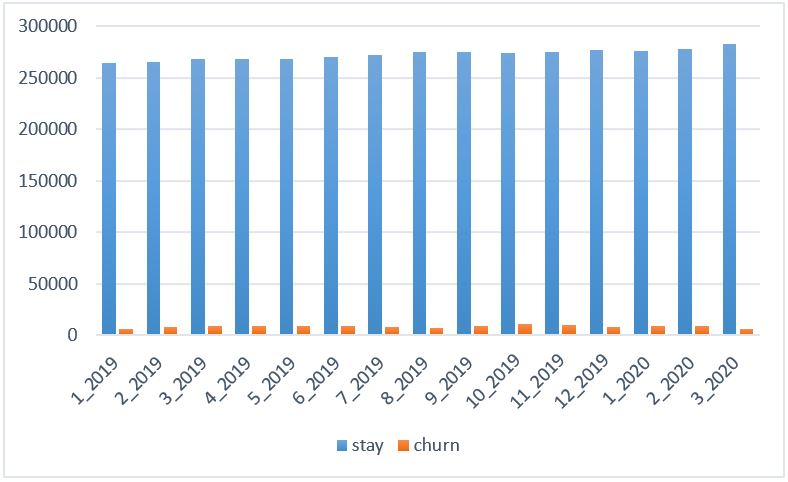
\includegraphics[width=0.50\textwidth]{images/distribution-over-months-small-medium.jpg}\label{fig:distribution-over-months-small-medium}}
  \caption{Data quantity distribution over the months}
\end{figure}

Imbalanced data can have a negative impact on the model performance. That is why the following two strategies have been implemented in order to provide a solution to this problem:

\subsubsection{Undersampling}

This method was used on the \textit{micro} training set which had around 16 000 000 observations for the over-represented class (the \textit{staying} class). The idea was to randomly sample approximately 5 000 000 observations from this class maintaining the original data distribution. To do so, a stratified sampling was implemented, grouping the data by \textit{year}, \textit{month} and \textit{churn}. An illustration of this process can be found in figure \ref{fig:undersampling-staying-class-micro}.

\begin{figure}[!ht]
    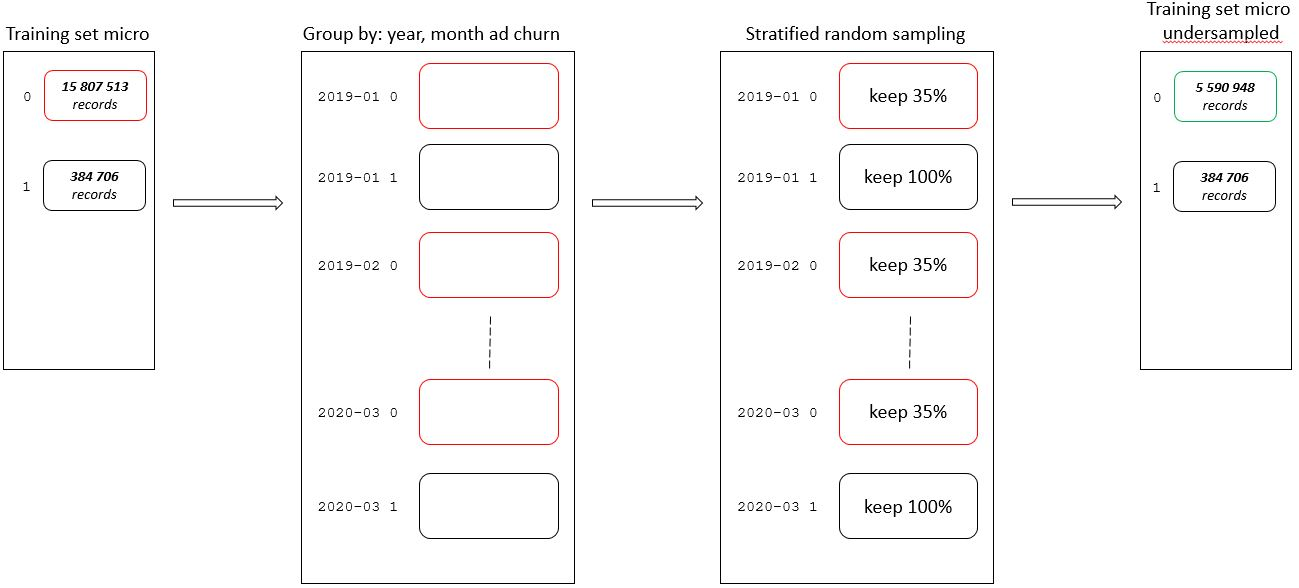
\includegraphics[width=0.95\textwidth]{images/undersampling-staying-class-micro.jpg}
    \centering
    \caption{Undersampling process of the \textit{staying} class: \textit{micro} data set}
    \label{fig:undersampling-staying-class-micro}
\end{figure}

\subsubsection{Oversampling}

This method instead was used in both \textit{micro} and \textit{small-medium} data sets. The goal was to increase the under-represented class (the \textit{churning} class) number of records up to approximately 5 000 000. This was achieved through the help of the \textit{pyspark} library. The idea of oversampling, is to duplicate the samples from the under-represented (1 in this case) class, to inflate the numbers till it reaches the same level as the dominant class (0 in this case).

Figures \ref{fig:balanced-distribution-over-months-micro} and \ref{fig:balanced-distribution-over-months-small-medium} show the new quantity distribution and we can clearly see the effects of undersampling and oversampling.

\begin{figure}[!ht]
  \centering
  \subfloat[Micro.]{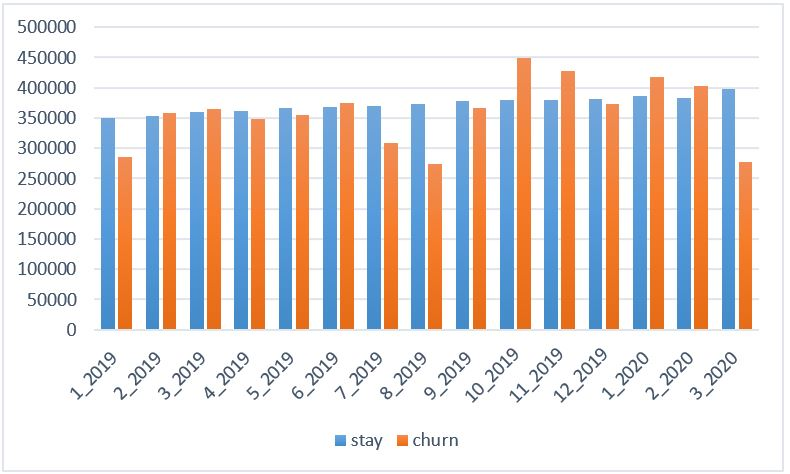
\includegraphics[width=0.50\textwidth]{images/balanced-distribution-over-months-micro.jpg}\label{fig:balanced-distribution-over-months-micro}}
  \hfill
  \subfloat[Small and Medium.]{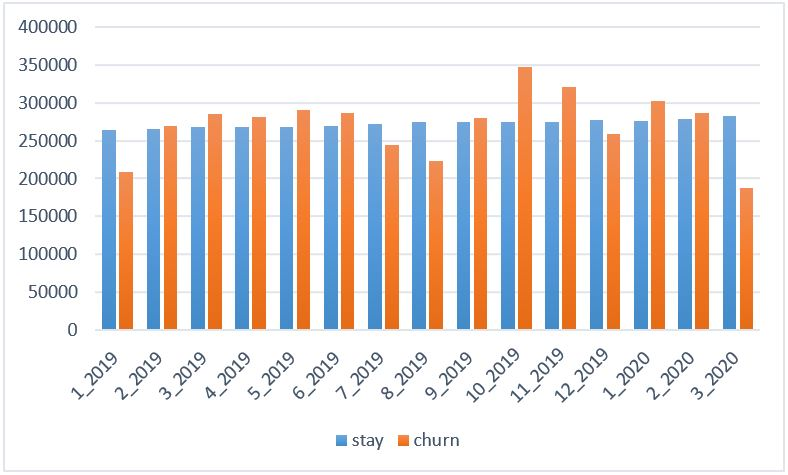
\includegraphics[width=0.50\textwidth]{images/balanced-distribution-over-months-small-medium.jpg}\label{fig:balanced-distribution-over-months-small-medium}}
  \caption{Balanced data: quantity distribution over the months}
\end{figure}

\subsection{Feature selection}

Feature selection is a crucial step of every machine learning project. Indeed, the training data set usually contains a lot of useless and noisy features that must be removed to allow the model to gain simplicity. As discussed in \ref{feature_selection}, multiple methods can used to achieve this goal. In the current section, we will discuss all the feature selection methods used in this study.

\subsubsection{Unique selector}

With this method, all the columns having only one unique value have been removed. Indeed, that kind of column contains no information that could be useful in predicting the target variable. 65 features have been removed from the \textit{micro} data set, while 68 have been removed from the \textit{small-medium} data set for this reason.

\subsubsection{Missing selector}

In this case, all the features having a missing value percentage higher than a given threshold have been removed. This kind of features can potentially add noise to the model predictions since most of the values are missing. Thus it is best to remove them. The threshold has been set to 60\% and 14 features have been removed from the \textit{micro} data set, while 12 have been removed from the \textit{small-medium} data set for this reason.

\subsubsection{Importance selector}

This method was used to drop features based on the feature importance of a gradient boosted tree model. Features were selected by their importance in such a way that the overall cumulative importance was equal to 0.99. With this method, 491 features were removed from the \textit{micro} data set and 459 from the \textit{small-medium} data set. Figures \ref{fig:cumulative-importance_vs_number-of-features_micro} and \ref{fig:cumulative-importance_vs_number-of-features_small-medium} show plots of the cumulative importance as a function of the number of features for both data sets in order to illustrate the importance selection process.

\begin{figure}[!ht]
  \centering
  \subfloat[Micro.]{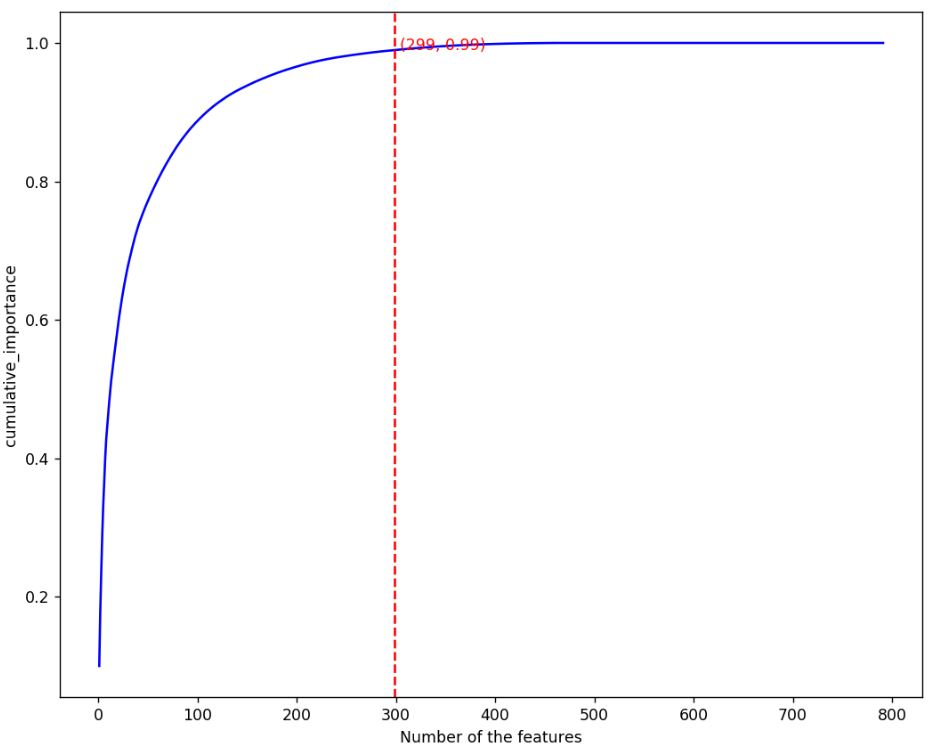
\includegraphics[width=0.50\textwidth]{images/cumulative-importance_vs_number-of-features_micro.jpg}\label{fig:cumulative-importance_vs_number-of-features_micro}}
  \hfill
  \subfloat[Small and Medium.]{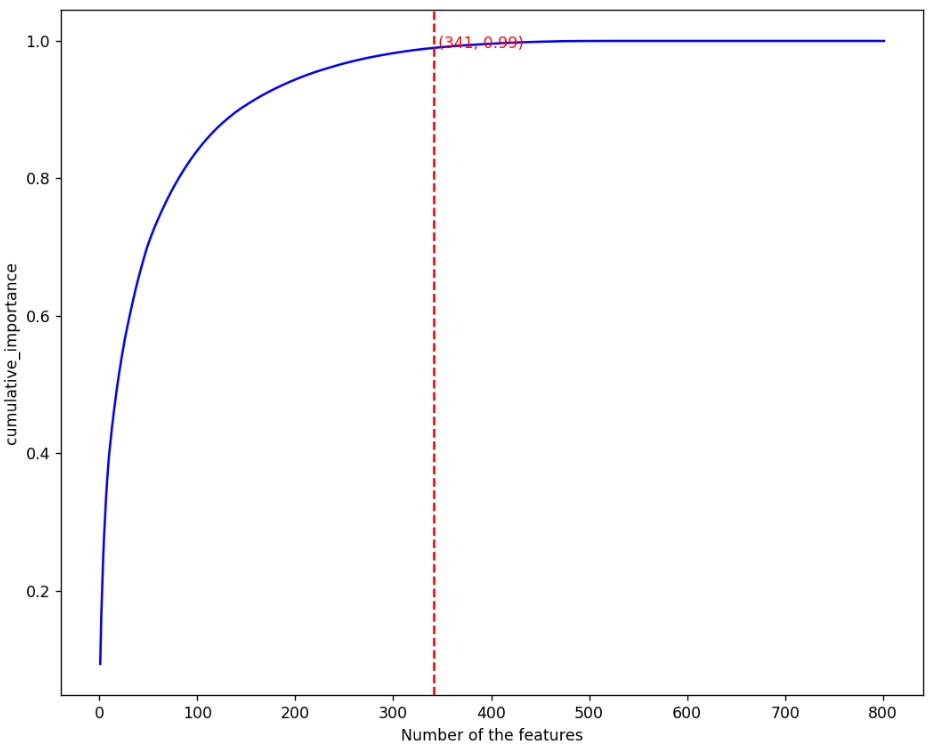
\includegraphics[width=0.50\textwidth]{images/cumulative-importance_vs_number-of-features_small-medium.jpg}\label{fig:cumulative-importance_vs_number-of-features_small-medium}}
  \caption{Cumulative importance vs number of features}
\end{figure}

\subsubsection{Correlation selector}

This is a very common feature selection method. We used it to identify and remove highly correlated features. A threshold was selected (0.9) and the pearson correlation metric was calculated among all the features. For all the couples of features having a pearson greater than 0.9, one of the features were removed. 63 features were removed for \textit{micro} and 81 features for \textit{small-medium}. Figures \ref{fig:correlation-matrix_micro} and \ref{fig:correlation-matrix_small-medium} show the plots of the correlation matrices built for the occasion.

\begin{figure}[!ht]
  \centering
  \subfloat[Micro.]{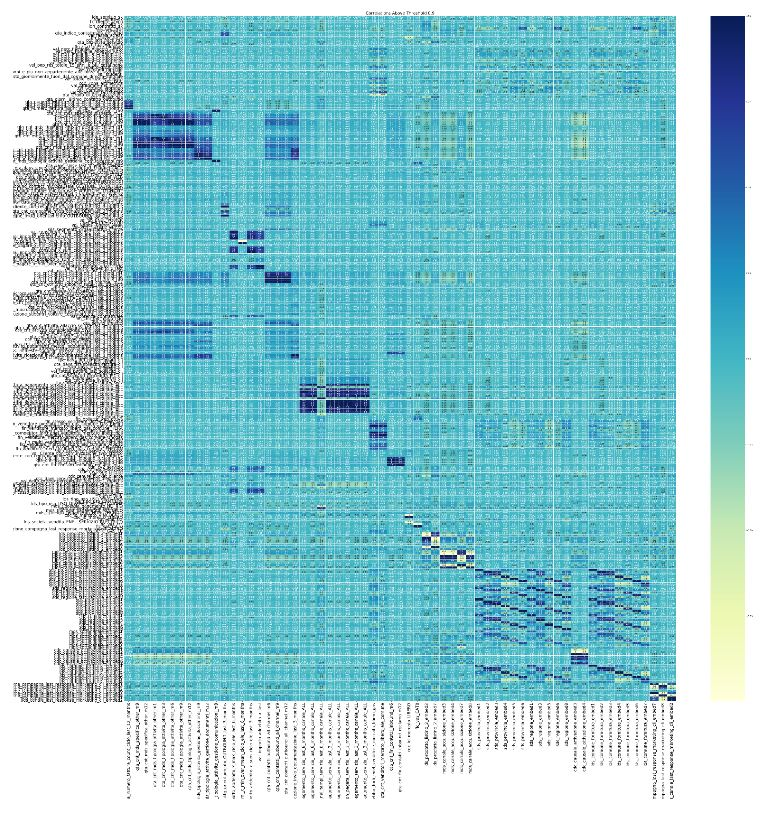
\includegraphics[width=0.50\textwidth]{images/correlation-matrix_micro.jpg}\label{fig:correlation-matrix_micro}}
  \hfill
  \subfloat[Small and Medium.]{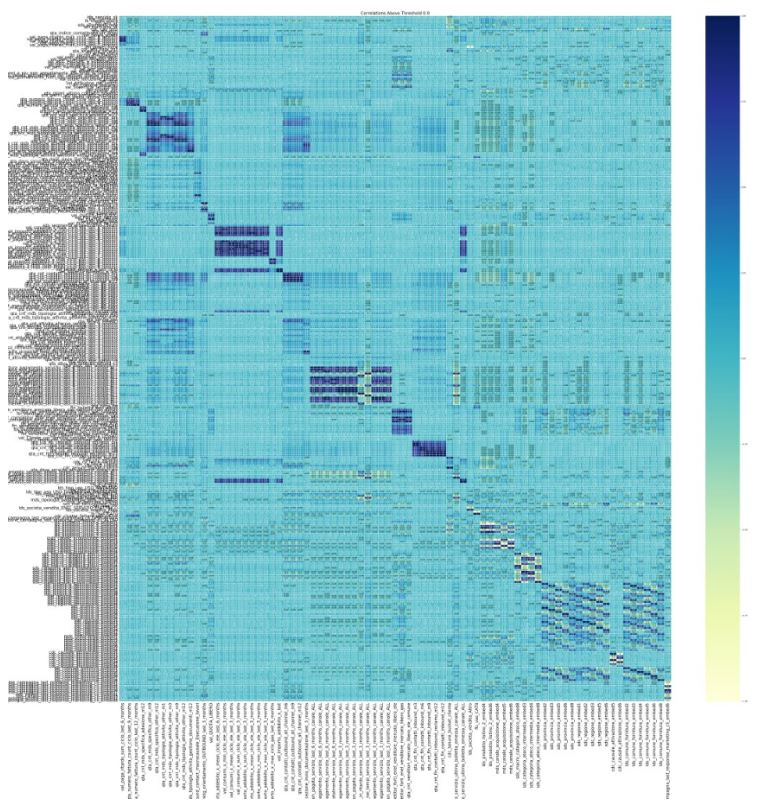
\includegraphics[width=0.50\textwidth]{images/correlation-matrix_small-medium.jpg}\label{fig:correlation-matrix_small-medium}}
  \caption{Correlation matrices}
\end{figure}

\subsubsection{Recursive feature elimination}

Recursive feature elimination (RFE) is a feature selection method that fits a model and removes the weakest feature (or features) until the specified number of features is reached. To find the optimal number of features, cross-validation is used with RFE to score different feature subsets and select the best scoring collection of features.\cite{scikitRFE}

In this study, we combined this method with a random forest classifier to identify the best collection of features to be used. The optimal and final number of features to be used was 49 for \textit{micro} and 55 for \textit{small-medium} as shown on figures \ref{fig:rfecv_micro} and \ref{fig:rfecv_small-medium} that plot f-score as a function of the number of selected features.

\begin{figure}[!ht]
  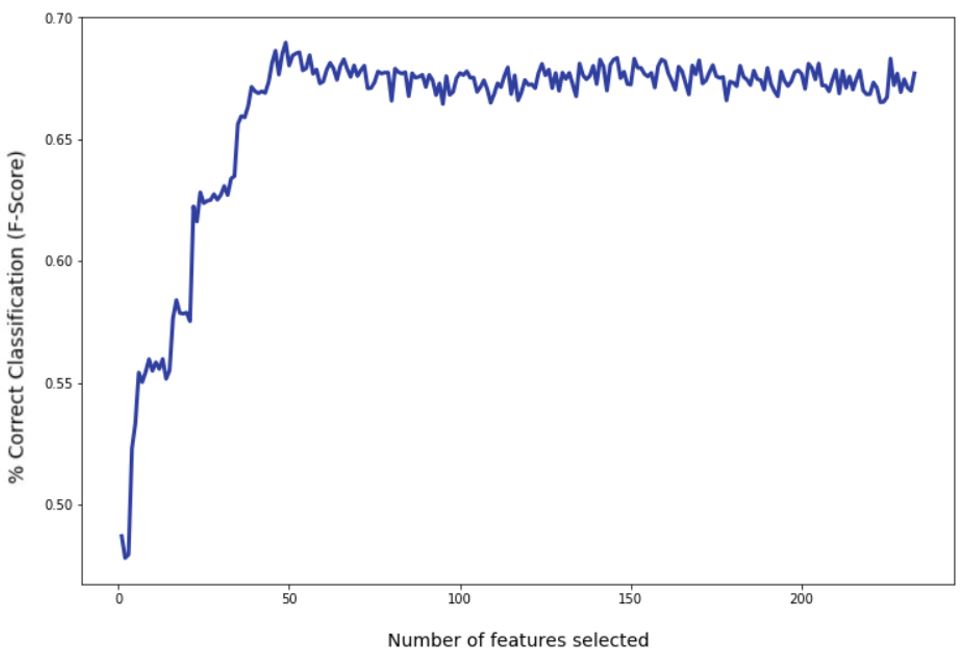
\includegraphics[width=0.95\textwidth]{images/rfecv_micro.jpg}
  \centering
  \caption{Recursive feature elimination with cross-validation: micro}	
  \label{fig:rfecv_micro}
\end{figure}

\begin{figure}[!ht]
  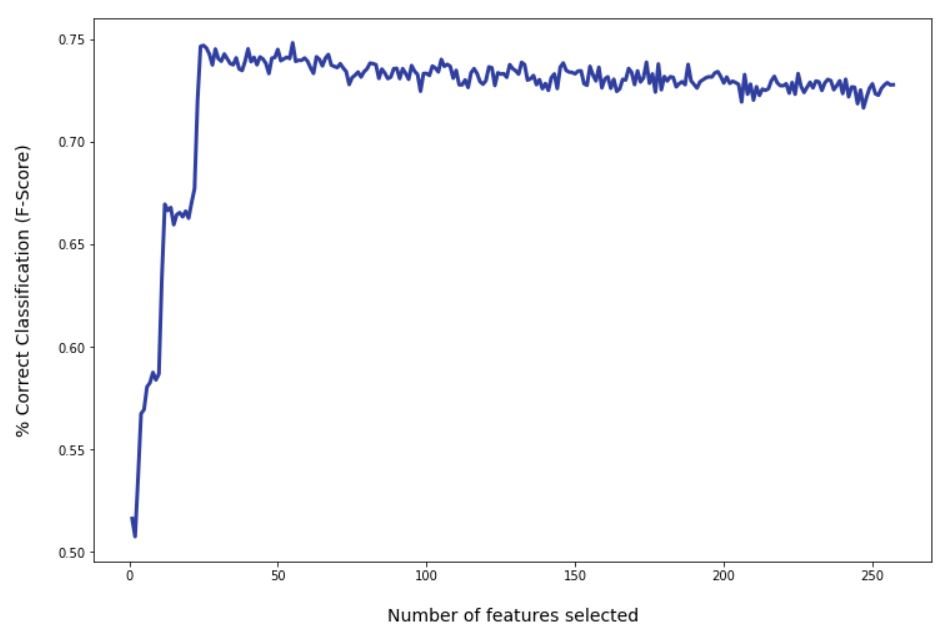
\includegraphics[width=0.95\textwidth]{images/rfecv_small-medium.jpg}
  \centering
  \caption{Recursive feature elimination with cross-validation: small-medium}
  \label{fig:rfecv_small-medium}
\end{figure}

\subsection{The complete workflow}

Figure \ref{fig:complete_wf} displays the complete workflow impleted in the this study starting from the data collection and ending with the transmission of the prediction to the marketing area for campaign.

\begin{figure}[!ht]
  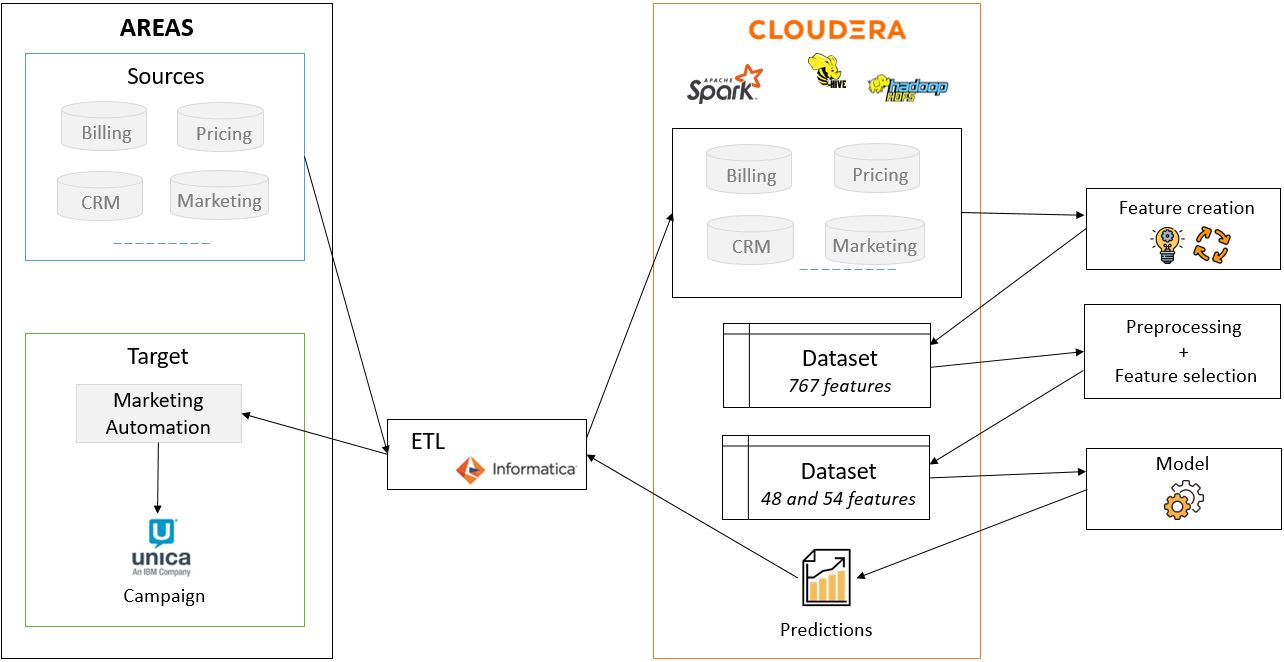
\includegraphics[width=0.95\textwidth]{images/complete_wf.jpg}
  \centering
  \caption{Complete workflow}
  \label{fig:complete_wf}
\end{figure}

\chapter{Models and results}

When speaking about machine learning and data science, people directly thing about modeling, which surprisingly is not the most tedious step of a data science project. However this phase is crucial and extremely important since it is where we use all the results obtained in the previous steps. It therefore clearly appears that this is a key phase, because if poorly implemented, it would make all the previous work useless.

In this chapter, we present all the machine learning models that we implemented during our experiment with the corresponding results. For each model, the following results are presented: (i) Precision, Recall, F-Measure, ROC AUC and PR AUC; (ii) The ROC curve and the PR curve; (iii) And finally the confusion matrices.

In the last part of this chapter, we compare all the models and present an optimized (through random search) version of the best performing one along with the final results.
  
\section{Logistic regression}

This model is often used as a baseline for binary classification problems. See section \ref{lr_model} for details. Some significant parameters for logistic regression are \textit{maxIter}, \textit{regParam}, \textit{elasticNetParam}, \textit{tol} and \textit{aggregationDepth}. (i) maxIter ($\ge 0$) represents the maximum number of iterations necessary for the solver to converge; (ii) regParam ($\ge 0$) is the regularization parameter; (iii) elasticNetParam is the \textit{ElasticNet} mixing parameter, in range $[0, 1]$. The used penalty changes based on the value of this parameter. An $L2$ penalty is used for for a value of $0$ while an $L1$ penalty is used for a value of $1$; (iv) tol ($\ge 0$) is the convergence tolerance for iterative algorithms; (v) aggregationDepth ($\ge 2$) represents the suggested depth for tree aggregate.\cite{pysparkLR}

The settings that we used with this model in \textit{pyspark}  for both data sets are the following: $maxIter = 50$, $regParam = 0.0$, $elasticNetParam = 0.0$, $tol = 1\mathrm{e}{-6}$ and $aggregationDepth = 2$. The obtained results are shown on table \ref{lr_metrics}. Figures \ref{fig:lr_roc_curve_micro} and \ref{fig:lr_roc_curve_small-medium} display the resulting ROC curves. Figures \ref{fig:lr_pr_curve_micro} and \ref{fig:lr_pr_curve_small-medium} show the PR curves. And finally, the resulting confusion matrices can be found on figures \ref{fig:lr_cm_micro} and \ref{fig:lr_cm_small-medium}.
 
\begin{table}[!ht]
\centering
\resizebox{\textwidth}{!}{
\begin{tabular}[t]{lcccccc}
\toprule
&Threshold&Precision (\%)&Recall (\%)&F1 Score (\%)&ROC AUC&PR AUC\\
\midrule
LR Micro&0.5&4.75846&59.0225&8.8069&0.704211&0.0756913\\
LR Small-Medium&0.5&5.61412&61.3749&10.2872&0.705553&0.0881378\\
\bottomrule
\end{tabular}
}
\vspace{2mm}
\caption{Logistic regression metrics}
\label{lr_metrics}
\end{table}

\begin{figure}[!ht]
  \centering
  \subfloat[Micro.]{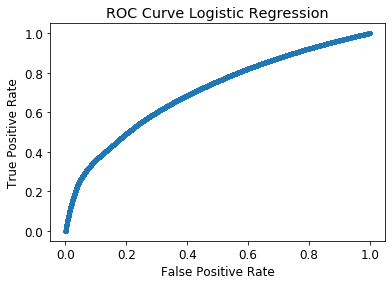
\includegraphics[width=0.50\textwidth]{images/lr_roc_curve_micro.png}\label{fig:lr_roc_curve_micro}}
  \hfill
  \subfloat[Small and Medium.]{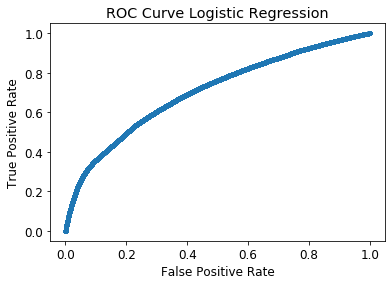
\includegraphics[width=0.50\textwidth]{images/lr_roc_curve_small-medium.png}\label{fig:lr_roc_curve_small-medium}}
  \caption{Logistic regression: ROC curves}
\end{figure}

\begin{figure}[!ht]
  \centering
  \subfloat[Micro.]{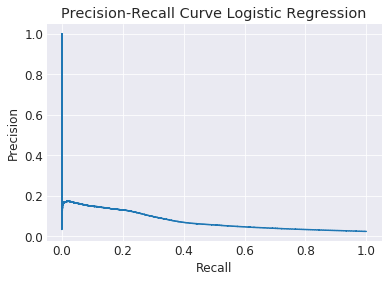
\includegraphics[width=0.50\textwidth]{images/lr_pr_curve_micro.png}\label{fig:lr_pr_curve_micro}}
  \hfill
  \subfloat[Small and Medium.]{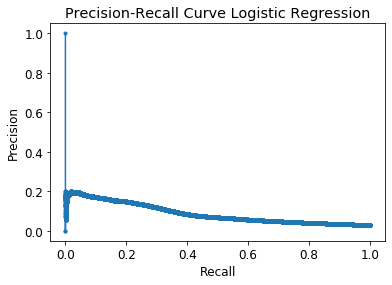
\includegraphics[width=0.50\textwidth]{images/lr_pr_curve_small-medium.png}\label{fig:lr_pr_curve_small-medium}}
  \caption{Logistic regression: PR curves}
\end{figure}

\begin{figure}[!ht]
  \centering
  \subfloat[Micro.]{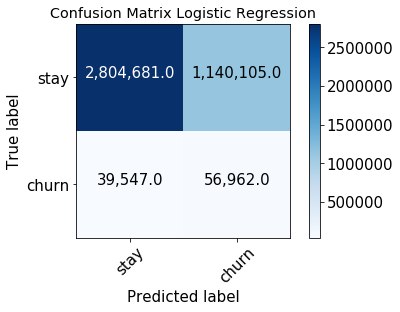
\includegraphics[width=0.50\textwidth]{images/lr_cm_micro.png}\label{fig:lr_cm_micro}}
  \hfill
  \subfloat[Small and Medium.]{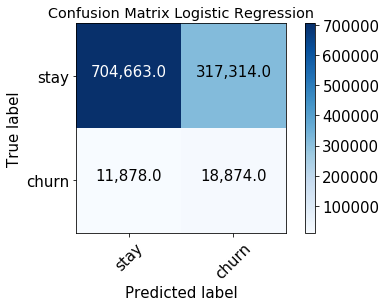
\includegraphics[width=0.50\textwidth]{images/lr_cm_small-medium.png}\label{fig:lr_cm_small-medium}}
  \caption{Logistic regression: Confusion matrices}
\end{figure}

\section{Decision tree classifier}

After logistic regression, we used decision tree classifier which is another simple model that, sometimes is also used as baseline in machine learning classification problems. Section \ref{dt_model} describes the logic behind this model. Let's take a look at the main parameters of this model: (i) \textit{maxDepth} ($\ge 0$) representing the maximum depth of the tree; (ii) \textit{maxBins} ($\ge 2$) is the maximum number of bins for discretizing continuous features; (iii) \textit{minInfoGain} which is the minimum information gain for a split to be considered at a tree node; (iv) \textit{impurity} which represents the criterion used for information gain calculation; The supported options are \textit{entropy} and  \textit{gini}; (v) \textit{minWeightFractionPerNode} ($[0.0, 0.5)$) which is the minimum fraction of the weighted sample count that each child must have after split.\cite{pysparkDT}

In \textit{pyspark}, the configuration that we used with this model both for small-medium and micro data sets is: $maxDepth = 5$, $maxBins = 32$, $minInfoGain = 0.0$, $impurity = gini$ and $minWeightFractionPerNode = 0.0$. Table \ref{dt_metrics} shows the obtained results on our data sets. Figures \ref{fig:dt_roc_curve_micro} and \ref{fig:dt_roc_curve_small-medium} display ROC curves while figures \ref{fig:dt_pr_curve_micro} and \ref{fig:dt_pr_curve_small-medium} show the PR curves. Finally, the confusion matrices are shown on figures \ref{fig:dt_cm_micro} and \ref{fig:dt_cm_small-medium} for both data sets.
 
\begin{table}[!ht]
\centering
\resizebox{\textwidth}{!}{
\begin{tabular}[t]{lcccccc}
\toprule
&Threshold&Precision (\%)&Recall (\%)&F1 Score (\%)&ROC AUC&PR AUC\\
\midrule
DT Micro&0.5&7.65107&44.4062&13.0531&0.689376&0.0916564\\
DT Small-Medium&0.5&7.76758&51.9121&13.5132&0.7147&0.0914786\\
\bottomrule
\end{tabular}
}
\vspace{2mm}
\caption{Decision tree classifier metrics}
\label{dt_metrics}
\end{table}

\begin{figure}[!ht]
  \centering
  \subfloat[Micro.]{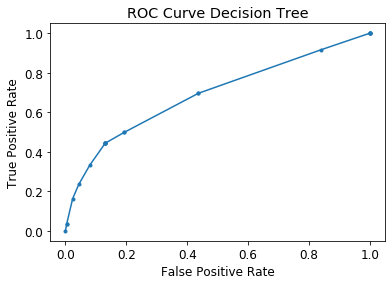
\includegraphics[width=0.50\textwidth]{images/dt_roc_curve_micro.png}\label{fig:dt_roc_curve_micro}}
  \hfill
  \subfloat[Small and Medium.]{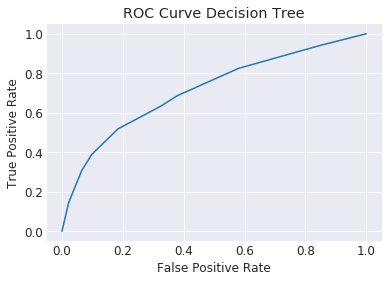
\includegraphics[width=0.50\textwidth]{images/dt_roc_curve_small-medium.png}\label{fig:dt_roc_curve_small-medium}}
  \caption{Decision tree classifier: ROC curves}
\end{figure}

\begin{figure}[!ht]
  \centering
  \subfloat[Micro.]{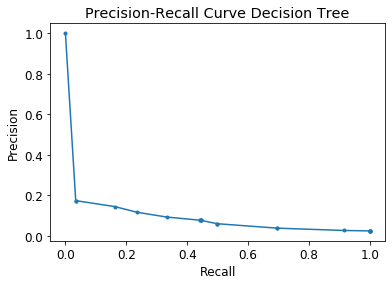
\includegraphics[width=0.50\textwidth]{images/dt_pr_curve_micro.png}\label{fig:dt_pr_curve_micro}}
  \hfill
  \subfloat[Small and Medium.]{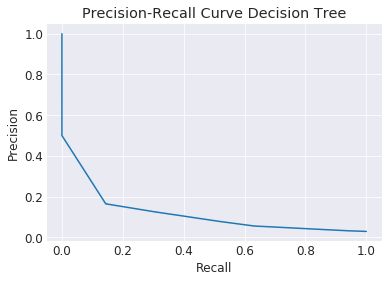
\includegraphics[width=0.50\textwidth]{images/dt_pr_curve_small-medium.png}\label{fig:dt_pr_curve_small-medium}}
  \caption{Decision tree classifier: PR curves}
\end{figure}

\begin{figure}[!ht]
  \centering
  \subfloat[Micro.]{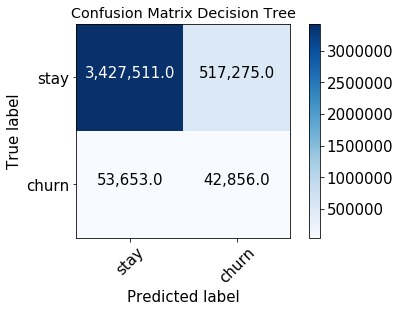
\includegraphics[width=0.50\textwidth]{images/dt_cm_micro.png}\label{fig:dt_cm_micro}}
  \hfill
  \subfloat[Small and Medium.]{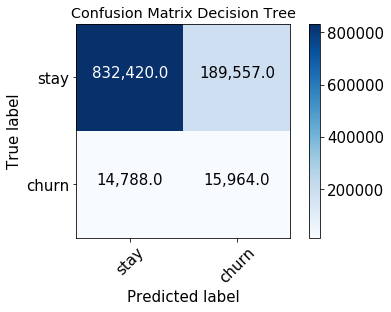
\includegraphics[width=0.50\textwidth]{images/dt_cm_small-medium.png}\label{fig:dt_cm_small-medium}}
  \caption{Decision tree classifier: Confusion matrices}
\end{figure}


\section{Random forest classifier}

Random forest classifier is another commonly used classifier that we adopted in our study. Section \ref{rf_model} gives more theoretical details about this model. Some of it's important parameters are: (i) \textit{maxDepth} and \textit{maxBins} are same as in decision tree; (ii) \textit{numTrees} ($\ge 1$) is the number of trees to train; (iv) \textit{subsamplingRate} ($(0, 1]$) represents the fraction of training data used for learning each decision tree.\cite{pysparkRF}

In \textit{pyspark}, the settings that we used with this model for our two data sets are: $maxDepth = 5$, $maxBins = 32$, $numTrees = 50$ and $subsamplingRate = 1.0$. The obtained results are shown on table \ref{rf_metrics}. Figures \ref{fig:rf_roc_curve_micro} and \ref{fig:rf_roc_curve_small-medium} display the ROC curves, figures \ref{fig:rf_pr_curve_micro} and \ref{fig:rf_pr_curve_small-medium} show the PR curves. And finally, figures \ref{fig:rf_cm_micro} and \ref{fig:rf_cm_small-medium} show the resulting confusion matrices.
 
\begin{table}[!ht]
\centering
\resizebox{\textwidth}{!}{
\begin{tabular}[t]{lcccccc}
\toprule
&Threshold&Precision (\%)&Recall (\%)&F1 Score (\%)&ROC AUC&PR AUC\\
\midrule
RF Micro&0.5&5.2842&56.1575&9.65948&0.716906&0.0798355\\
RF Small-Medium&0.5&5.53378&64.5486&10.1937&0.727238&0.0975543\\
\bottomrule
\end{tabular}
}
\vspace{2mm}
\caption{Random forest classifier metrics}
\label{rf_metrics}
\end{table}

\begin{figure}[!ht]
  \centering
  \subfloat[Micro.]{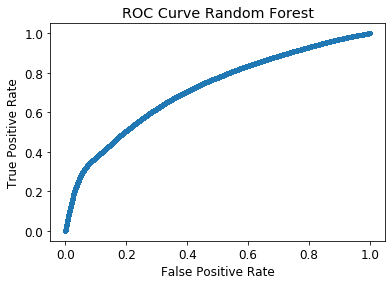
\includegraphics[width=0.50\textwidth]{images/rf_roc_curve_micro.png}\label{fig:rf_roc_curve_micro}}
  \hfill
  \subfloat[Small and Medium.]{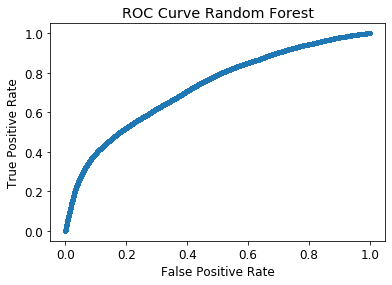
\includegraphics[width=0.50\textwidth]{images/rf_roc_curve_small-medium.png}\label{fig:rf_roc_curve_small-medium}}
  \caption{Random forest classifier: ROC curves}
\end{figure}

\begin{figure}[!ht]
  \centering
  \subfloat[Micro.]{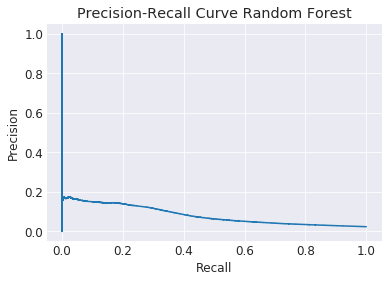
\includegraphics[width=0.50\textwidth]{images/rf_pr_curve_micro.png}\label{fig:rf_pr_curve_micro}}
  \hfill
  \subfloat[Small and Medium.]{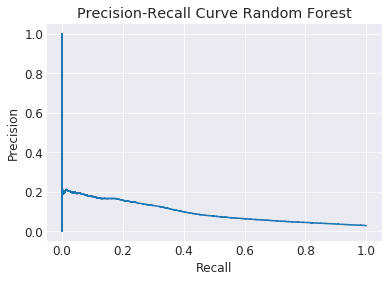
\includegraphics[width=0.50\textwidth]{images/rf_pr_curve_small-medium.png}\label{fig:rf_pr_curve_small-medium}}
  \caption{Random forest classifier: PR curves}
\end{figure}

\begin{figure}[!ht]
  \centering
  \subfloat[Micro.]{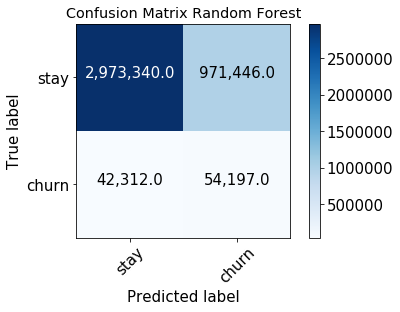
\includegraphics[width=0.50\textwidth]{images/rf_cm_micro.png}\label{fig:rf_cm_micro}}
  \hfill
  \subfloat[Small and Medium.]{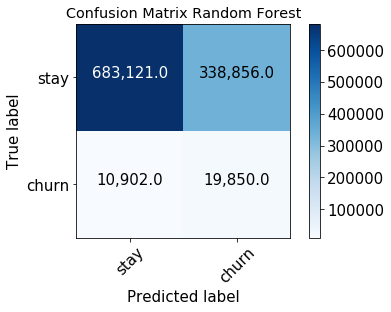
\includegraphics[width=0.50\textwidth]{images/rf_cm_small-medium.png}\label{fig:rf_cm_small-medium}}
  \caption{Random forest classifier: Confusion matrices}
\end{figure}


\section{Gradient-boosted tree classifier}

As already introduced in section \ref{boosting_model}, this model is one of the most commonly used boosting techniques. It used gradient descent to minimize the loss function. This model has been adopted in this study, in order to improve the results of simpler models like logistic regression and decision tree classifier. Indeed we obtained quite better results. Some important parameters of this model are the following: (i) \textit{maxDepth}, \textit{maxBins}, \textit{minInfoGain}, \textit{maxIter} and \textit{subsamplingRate} with the same meaning as for the previous models (Decision tree and Random forest); (ii) \textit{lossType} is the loss function that the GBT model tries to minimize; (iii) \textit{stepSize} ($(0, 1]$) represents the step size also known as learning rate for shrinking the contribution of each estimator; (iv) \textit{impurity} is the criterion used for information gain calculation.\cite{pysparkGBT}

We used \textit{pyspark} with the following settings to implement this model: $maxDepth = 5$, $maxBins = 32$, $minInfoGain = 0.0$, $lossType = logistic$, $maxIter = 50$, $stepSize = 0.1$, $subsamplingRate = 1.0$ and $impurity = variance$. The obtained results can be found on table \ref{gbt_metrics}. Figures \ref{fig:gbt_roc_curve_micro} and \ref{fig:gbt_roc_curve_small-medium} display the ROC curves, figures \ref{fig:gbt_pr_curve_micro} and \ref{fig:gbt_pr_curve_small-medium} show the PR curves. And finally, figures \ref{fig:gbt_cm_micro} and \ref{fig:gbt_cm_small-medium} show the resulting confusion matrices of the implemented model.
 
\begin{table}[!ht]
\centering
\resizebox{\textwidth}{!}{
\begin{tabular}[t]{lcccccc}
\toprule
&Threshold&Precision (\%)&Recall (\%)&F1 Score (\%)&ROC AUC&PR AUC\\
\midrule
GBT Micro&0.5&6.21126&62.904&11.3061&0.772177&0.104269\\
GBT Small-Medium&0.5&7.32602&69.5662&13.256&0.794414&0.138775\\
\bottomrule
\end{tabular}
}
\vspace{2mm}
\caption{Gradient-boosted tree classifier metrics}
\label{gbt_metrics}
\end{table}

\begin{figure}[!ht]
  \centering
  \subfloat[Micro.]{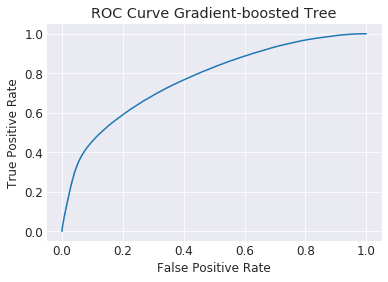
\includegraphics[width=0.50\textwidth]{images/gbt_roc_curve_micro.png}\label{fig:gbt_roc_curve_micro}}
  \hfill
  \subfloat[Small and Medium.]{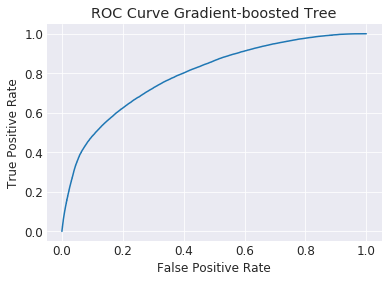
\includegraphics[width=0.50\textwidth]{images/gbt_roc_curve_small-medium.png}\label{fig:gbt_roc_curve_small-medium}}
  \caption{Gradient-boosted tree classifier: ROC curves}
\end{figure}

\begin{figure}[!ht]
  \centering
  \subfloat[Micro.]{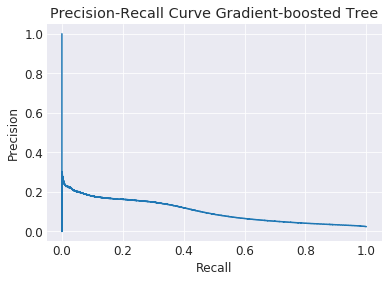
\includegraphics[width=0.50\textwidth]{images/gbt_pr_curve_micro.png}\label{fig:gbt_pr_curve_micro}}
  \hfill
  \subfloat[Small and Medium.]{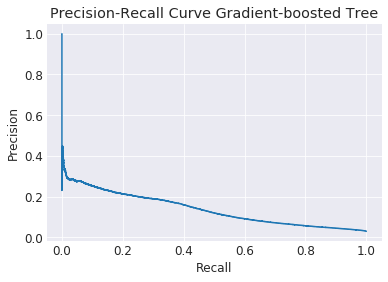
\includegraphics[width=0.50\textwidth]{images/gbt_pr_curve_small-medium.png}\label{fig:gbt_pr_curve_small-medium}}
  \caption{Gradient-boosted tree classifier: PR curves}
\end{figure}

\begin{figure}[!ht]
  \centering
  \subfloat[Micro.]{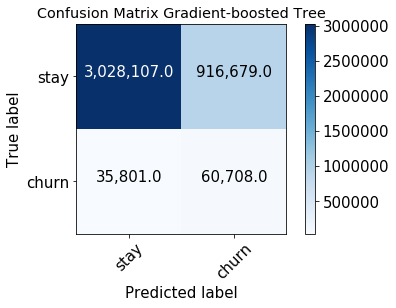
\includegraphics[width=0.50\textwidth]{images/gbt_cm_micro.png}\label{fig:gbt_cm_micro}}
  \hfill
  \subfloat[Small and Medium.]{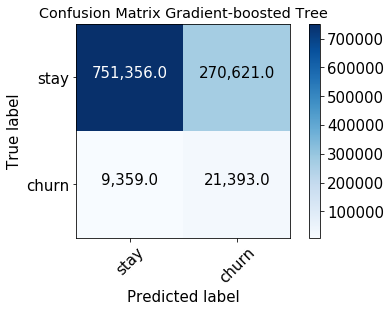
\includegraphics[width=0.50\textwidth]{images/gbt_cm_small-medium.png}\label{fig:gbt_cm_small-medium}}
  \caption{Gradient-boosted tree classifier: Confusion matrices}
\end{figure}

\section{XGBoost}

One of the major inefficiencies in gradient boosting is that the process of creating the trees is sequential (namely it creates one decision tree at a time). XGBoost (Extreme Gradient Boosting) is a model that was introduced by Tianqi Chen and Carlos Guestrin to overcome this inefficiency.\cite{Tianqi2016}

The results that we obtained with this model are shown on table \ref{xgb_metrics}. Figures \ref{fig:xgb_roc_curve_micro} and \ref{fig:xgb_roc_curve_small-medium} display the ROC curves, figures \ref{fig:xgb_pr_curve_micro} and \ref{fig:xgb_pr_curve_small-medium} show the PR curves. And finally, figures \ref{fig:xgb_cm_micro} and \ref{fig:xgb_cm_small-medium} show the resulting confusion matrices.
 
\begin{table}[!ht]
\centering
\resizebox{\textwidth}{!}{
\begin{tabular}[t]{lcccccc}
\toprule
&Threshold&Precision (\%)&Recall (\%)&F1 Score (\%)&ROC AUC&PR AUC\\
\midrule
XGB Micro&0.5&7.15468&57.0475&12.7147&0.769127&0.103214\\
XGB Small-Medium&0.5&7.85845&62.2334&13.9548&0.778677&0.124997\\
\bottomrule
\end{tabular}
}
\vspace{2mm}
\caption{XGBoost metrics}
\label{xgb_metrics}
\end{table}

\begin{figure}[!ht]
  \centering
  \subfloat[Micro.]{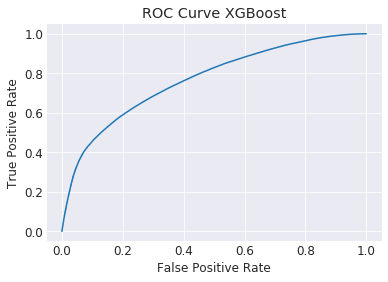
\includegraphics[width=0.50\textwidth]{images/xgb_roc_curve_micro.png}\label{fig:xgb_roc_curve_micro}}
  \hfill
  \subfloat[Small and Medium.]{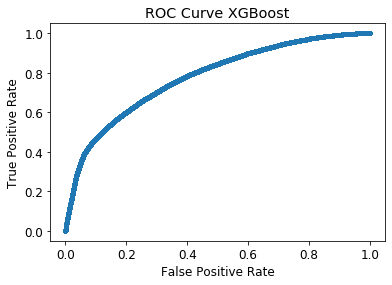
\includegraphics[width=0.50\textwidth]{images/xgb_roc_curve_small-medium.png}\label{fig:xgb_roc_curve_small-medium}}
  \caption{XGBoost: ROC curves}
\end{figure}

\begin{figure}[!ht]
  \centering
  \subfloat[Micro.]{\includegraphics[width=0.50\textwidth]{images/xgb_pr_curve_micro.png}\label{fig:xgb_pr_curve_micro}}
  \hfill
  \subfloat[Small and Medium.]{\includegraphics[width=0.50\textwidth]{images/xgb_pr_curve_small-medium.png}\label{fig:xgb_pr_curve_small-medium}}
  \caption{XGBoost: PR curves}
\end{figure}

\begin{figure}[!ht]
  \centering
  \subfloat[Micro.]{\includegraphics[width=0.50\textwidth]{images/xgb_cm_micro.png}\label{fig:xgb_cm_micro}}
  \hfill
  \subfloat[Small and Medium.]{\includegraphics[width=0.50\textwidth]{images/xgb_cm_small-medium.png}\label{fig:xgb_cm_small-medium}}
  \caption{XGBoost: Confusion matrices}
\end{figure}


\section{Summary and analysis of the results}

In summary, 5 different machine learning models were used in this study (Logistic regression, Random forest, Decision tree, Gradient-boosted tree and XGBoost) to predict customer churn. These 5 models have been evaluated using 6 different evaluation metrics (Confusion matrix, Precision, Recall, F1 Score, ROC AUC and PR AUC). To choose the best performing model, we focused our attention on precision and recall since we were interested by both the quality and the quantity of the positive predictions. F1 Score is as combination of this two metrics. 

However the initial predictions were made using the default threshold (0.5); Thus, it was then necessary to find a metric able to summarize the model performance over all the possible thresholds so that the best threshold could then be identified. Precision and Recall area under the curve (PR AUC) was thought to be the right metric to do so.

As shown on tables \ref{results_summary_micro} and \ref{results_summary_small-medium}, the best model appears to be \textit{Gradient Boosted Tree Classifier} with a PR AUC of approximately $0.10$ for \textit{micro} and $0.13$ for textit{small-medium} data sets. 


\begin{table}[!ht]
\centering
\resizebox{\textwidth}{!}{
\begin{tabular}[t]{lcccccc}
\toprule
&Threshold&Precision (\%)&Recall (\%)&F1 Score (\%)&ROC AUC&PR AUC\\
\midrule
LR Micro&0.5&4.75846&59.0225&8.8069&0.704211&0.0756913\\
DT Micro&0.5&7.65107&44.4062&13.0531&0.689376&0.0916564\\
RF Micro&0.5&5.2842&56.1575&9.65948&0.716906&0.0798355\\
GBT Micro&0.5&6.21126&62.904&11.3061&0.772177&0.104269\\
XGB Micro&0.5&7.15468&57.0475&12.7147&0.769127&0.103214\\
\bottomrule
\end{tabular}
}
\vspace{2mm}
\caption{Results summary (Micro)}
\label{results_summary_micro}
\end{table}

\begin{table}[!ht]
\centering
\resizebox{\textwidth}{!}{
\begin{tabular}[t]{lcccccc}
\toprule
&Threshold&Precision (\%)&Recall (\%)&F1 Score (\%)&ROC AUC&PR AUC\\
\midrule
LR Small-Medium&0.5&5.61412&61.3749&10.2872&0.705553&0.0881378\\
DT Small-Medium&0.5&7.76758&51.9121&13.5132&0.7147&0.0914786\\
RF Small-Medium&0.5&5.53378&64.5486&10.1937&0.727238&0.0975543\\
GBT Small-Medium&0.5&7.32602&69.5662&13.256&0.794414&0.138775\\
XFB Small-Medium&0.5&7.85845&62.2334&13.9548&0.778677&0.124997\\
\bottomrule
\end{tabular}
}
\vspace{2mm}
\caption{Results summary (Small-medium)}
\label{results_summary_small-medium}
\end{table}

Some more work has been conducted in order to further optimize the best performing model including, parameter tuning through random search and threshold optimization. 

\subsection{Random search}

Parameter tuning is a very important step in machine learning, since it helps in improving the model performances. In this experiment, we ran a random search on a set of 7 parameters in order to identify the set of parameters yielding the best model. Tables \ref{results_random_search_micro} and \ref{results_random_search_small-medium} display the best obtained parameters for our two data sets. The best performances were obtained at iteration 11 for micro and 15 for small-medium as shown on figures \ref{fig:rendom_search_micro} and \ref{fig:rendom_search_small-medium}. These 2 figures show plots of the PR AUC as a function of the iterations.

\begin{table}[!ht]
\resizebox{\textwidth}{!}{
\begin{minipage}{.6\textwidth}
\centering
\begin{tabular}[t]{lc}
\toprule
Parameter&Value\\
\midrule
maxDepth&18\\
maxBins&10\\
minInstancesPerNode&9\\
checkpointInterval&4\\
maxIter&29\\
stepSize&0.4656094697539778\\
subsamplingRate&0.9676665353677678\\
\bottomrule
\end{tabular}
\vspace{2mm}
\caption{Random search results (Micro)}
\label{results_random_search_micro}
\end{minipage}
\hfill
\begin{minipage}{.6\textwidth}
\centering
\begin{tabular}[t]{lc}
\toprule
Parameter&Value\\
\midrule
maxDepth&19\\
maxBins&3\\
minInstancesPerNode&4\\
checkpointInterval&6\\
maxIter&18\\
stepSize&0.12112833339583066\\
subsamplingRate&0.6956739102219601\\
\bottomrule
\end{tabular}
\vspace{2mm}
\caption{Random search results (Small-Medium)}
\label{results_random_search_small-medium}
\end{minipage}
}
\end{table}

\begin{figure}[!ht]
  \centering
  \subfloat[Micro.]{\includegraphics[width=0.50\textwidth]{images/random_search_micro.jpg}\label{fig:rendom_search_micro}}
  \hfill
  \subfloat[Small and Medium.]{\includegraphics[width=0.50\textwidth]{images/random_search_small-medium.jpg}\label{fig:rendom_search_small-medium}}
  \caption{Random search - PR AUC by iteration}
\end{figure}


\subsection{Threshold optimization and final results}

Running the gradient boosted tree model with the best parameters identified in the previous step through random search, we obtained the final results with the default threshold ($0.5$). Moreover threshold optimization process has been made to identify the threshold yielding the best performances. Threshold optimization was performed using both ROC and PR curves. The final ROC curves can be found on figures \ref{fig:gbt_final_roc_curve_micro} and \ref{fig:gbt_final_roc_curve_small-medium}. The final PR curves are displayed on figures \ref{fig:gbt_final_pr_curve_micro} and \ref{fig:gbt_final_roc_curve_small-medium}. Figures \ref{fig:gbt_final_cm_micro} and \ref{fig:gbt_final_cm_small-medium} show the confusion matrices for different thresholds and for our two data sets. Figures \ref{fig:gbt_final_feature_importance_micro} and \ref{fig:gbt_final_feature_importance_small-medium} display the first 10 most important features of the final model. And lastly, the final results are summarized in table \ref{final_results_summary}.

\begin{figure}[!ht]
  \centering
  \subfloat[Micro.]{\includegraphics[width=0.50\textwidth]{images/gbt_final_roc_curve_micro.png}\label{fig:gbt_final_roc_curve_micro}}
  \hfill
  \subfloat[Small and Medium.]{\includegraphics[width=0.50\textwidth]{images/gbt_final_roc_curve_small-medium.png}\label{fig:gbt_final_roc_curve_small-medium}}
  \caption{GBT - Final ROC curves}
\end{figure}


\begin{figure}[!ht]
  \centering
  \subfloat[Micro.]{\includegraphics[width=0.50\textwidth]{images/gbt_final_pr_curve_micro.png}\label{fig:gbt_final_pr_curve_micro}}
  \hfill
  \subfloat[Small and Medium.]{\includegraphics[width=0.50\textwidth]{images/gbt_final_pr_curve_small-medium.png}\label{fig:gbt_final_pr_curve_small-medium}}
  \caption{GBT - Final PR curves}
\end{figure}


\begin{figure}[!ht]
  \centering
  \subfloat[Default threshold.]{\includegraphics[width=0.33\textwidth]{images/gbt_final_cm_default_th_micro.png}\label{fig:gbt_final_cm_default_th_micro}}
  \hfill
  \subfloat[ROC curve: Best th.]{\includegraphics[width=0.33\textwidth]{images/gbt_final_cm_best_roc_th_micro.png}\label{fig:gbt_final_cm_best_roc_th_micro}}
  \hfill
  \subfloat[PR curve : Best th.]{\includegraphics[width=0.33\textwidth]{images/gbt_final_cm_best_pr_th_micro.png}\label{fig:gbt_final_cm_best_pr_th_micro}}
  \caption{Micro: Confusion matrices for three different thresholds}
  \label{fig:gbt_final_cm_micro}
\end{figure}

\begin{figure}[!ht]
  \centering
  \subfloat[Default threshold.]{\includegraphics[width=0.33\textwidth]{images/gbt_final_cm_default_th_small-medium.png}\label{fig:gbt_final_cm_default_th_small-medium}}
  \hfill
  \subfloat[ROC curve: Best th.]{\includegraphics[width=0.33\textwidth]{images/gbt_final_cm_best_roc_th_small-medium.png}\label{fig:gbt_final_cm_best_roc_th_small-medium}}
  \hfill
  \subfloat[PR curve : Best th.]{\includegraphics[width=0.33\textwidth]{images/gbt_final_cm_best_pr_th_small-medium.png}\label{fig:gbt_final_cm_best_pr_th_small-medium}}
  \caption{Small-Medium: Confusion matrices for three different thresholds}
  \label{fig:gbt_final_cm_small-medium}
\end{figure}

\begin{figure}[!ht]
  \centering
  \subfloat[Micro.]{\includegraphics[width=0.50\textwidth]{images/gbt_final_feature_importance_micro.jpg}\label{fig:gbt_final_feature_importance_micro}}
  \hfill
  \subfloat[Small and Medium.]{\includegraphics[width=0.50\textwidth]{images/gbt_final_feature_importance_small-medium.jpg}\label{fig:gbt_final_feature_importance_small-medium}}
  \caption{GBT - Feature importance}
\end{figure}

\begin{table}[!htb]
\centering
\resizebox{\textwidth}{!}{
\begin{tabular}[t]{lcccccc}
\toprule
&Threshold&Precision (\%)&Recall (\%)&F1 Score (\%)&ROC AUC&PR AUC\\
\midrule
GBT Micro (Default th.)&0.5&20.0593&36.4681	&25.8821&0.809498&0.192311\\
GBT Micro (ROC best th.)&0.0928788&7.55362&69.5023&13.6263&0.809498&0.192311\\
GBT Micro (PR best th.)&0.617549&24.5504&29.819&26.9294&0.809498&0.192311\\
GBT Small-Medium (Default th.)&0.5&35.2695&63.0268&45.229&0.886273&0.532811\\
GBT Small-Medium (ROC best th.)&0.302107&18.0879&72.8668&28.9816&0.886273&0.532811\\
GBT Small-Medium (PR best th.)&0.697076&63.9946&48.0522&54.8892&0.886273&0.532811\\
\bottomrule
\end{tabular}
}
\vspace{2mm}
\caption{Final model results for different thresholds}
\label{final_results_summary}
\end{table}


\chapter{Conclusions}

\section{Conclusion}

The goal of this experiment was to build a model able to accurately predict the churn probability of a given client. Such a model brings a sure competitive advantage for an energy provider since this makes it possible to take necessary actions in order to retain critical clients. There is no standard model to accurately address this issue, that is why we tried different techniques in this study.

The first step of the study consisted in collecting from various company areas the data necessary to the modeling phase. To do so, some ETL processes were implemented to move the data from several company areas into a dedicated cluster (Data Lake). In this cluster the data was aggregated in a feature creation phase where we generated 767 features and a data set containing 15 months (from January 2019 to March 2020). As required by the company, the data was divided in two groups based on the size of the corresponding client (micro and small-medium). The generated data sets were made up of more than 20 millions observations for the micro clients against 5 millions for the small and medium clients.

Subsequently, some preprocessing tasks were realized in order to appropriately prepare the data to the modeling phase. Among those tasks we have missing data handling (Imputation by a neutral value, Imputation by a new value), categorical features encoding (one-hot, boolean, ordinal, embeddings), imbalanced data handling (under and over sampling) and feature selection (unique selector, missing selector,importance selector, correlation selector and recursive feature elimination). After the preprocessing phase, we obtained two cleaned data sets with 48 features for micro and 54 features for small-medium. These data sets were then split into two sets for each cluster: Train (80\%) and Test (20\%).

Lastly, several models were implemented. the two best performing models appeared to be Gradient Boosted Tree (PR AUC = 0.1042 before optimization) and XGBoost (PR AUC = 0.1032 before optimization) with GBT performing slightly better than XGBoost. The fact that these two models turned out to be the best performing ones was not a big surprise for us because our data sets were big and complex. Indeed, tree based models are known to be good at handling complex and non-linear relationships among features.

After optimizing the best model (Gradient Boosted Tree), we obtained a precision of 25\%, and a recall of 30\% on the cluster of micro clients and a precision of 64\% and a recall of 48\% on the cluster of small-medium clients. Given the huge amount of training and testing data used, we can say that these results are quite good and this model could be considered as a good starting point for further research on churn prediction in energy field.

\section{Suggestion for future research}

Knowing in advance when a client is about to churn is certainly very important since it could help in taking effective actions to reverse the process and retain that client. However to identify the right action to be taken, the reason why the client is churning could be very helpful. Analyzing these reasons could be an excellent subject for a future research.

\backmatter

\cleardoublepage
\phantomsection % Give this command only if hyperref is loaded
\addcontentsline{toc}{chapter}{\bibname}
\begin{thebibliography}{9}

\bibitem{Geron2017} 
Aurélien Géron (13 March 2017). \href{https://books.google.com/books?id=bRpYDgAAQBAJ}{Hands-On Machine Learning with Scikit-Learn and TensorFlow: Concepts, Tools, and Techniques to Build Intelligent Systems}. O'Reilly Media. ISBN 978-1-4919-6224-4.

\bibitem{Sousa2015} 
Eusébio E., de Sousa J., Ventim Neves M. (2015). \href{https://doi.org/10.1007/978-3-319-16766-4_39}{Risk Analysis and Behavior of Electricity Portfolio Aggregator}. In: Camarinha-Matos L., Baldissera T., Di Orio G., Marques F. (eds) Technological Innovation for Cloud-Based Engineering Systems. DoCEIS 2015. IFIP Advances in Information and Communication Technology, vol 450. Springer, Cham.

\bibitem{Garcia2016} 
Martínez García I.E., Sánchez A.S., Barbati S. (2016). \href{https://doi.org/10.1007/978-3-319-39095-6_15}{Reliability and Preventive Maintenance}. In: Ostachowicz W., McGugan M., Schröder-Hinrichs JU., Luczak M. (eds) MARE-WINT. Springer, Cham.

\bibitem{Awad2015} 
Awad M., Khanna R. (2015). \href{https://doi.org/10.1007/978-1-4302-5990-9_1}{Machine Learning}. In: Efficient Learning Machines. Apress, Berkeley, CA.

\bibitem{Vassiliadis2002}
Vassiliadis P., Simitsis A., Skiadopoulos S. (2002). \href{https://doi.org/10.1007/3-540-47961-9_67}{On the Logical Modeling of ETL Processes}. In: Pidduck A.B., Ozsu M.T., Mylopoulos J., Woo C.C. (eds) Advanced Information Systems Engineering. CAiSE 2002. Lecture Notes in Computer Science, vol 2348. Springer, Berlin, Heidelberg.

\bibitem{Capuccini2017}
Capuccini, M., Ahmed, L., Schaal, W. et al. \href{https://doi.org/10.1007/3-540-47961-9_67}{Large-scale virtual screening on public cloud resources with Apache Spark}. J Cheminform 9, 15 (2017).

\bibitem{Salgado2016}
Salgado C.M., Azevedo C., Proença H., Vieira S.M. (2016). \href{https://doi.org/10.1007/978-3-319-43742-2_13}{Missing Data}. In: Secondary Analysis of Electronic Health Records. Springer, Cham.

\bibitem{Barandela2004}
Barandela R., Valdovinos R.M., Sánchez J.S., Ferri F.J. (2004). \href{https://doi.org/10.1007/978-3-540-27868-9_88}{The Imbalanced Training Sample Problem: Under or over Sampling?}. In: Fred A., Caelli T.M., Duin R.P.W., Campilho A.C., de Ridder D. (eds) Structural, Syntactic, and Statistical Pattern Recognition. SSPR /SPR 2004. Lecture Notes in Computer Science, vol 3138. Springer, Berlin, Heidelberg.

\bibitem{Hancock2020}
Hancock, J.T., Khoshgoftaar, T.M. \href{https://doi.org/10.1186/s40537-020-00305-w}{Survey on categorical data for neural networks}. J Big Data 7, 28 (2020).

\bibitem{Almeida2019}
F. Almeida and G. Xexeo \href{http://arxiv.org/abs/1901.09069}{Word embeddings: A survey}. CoRR, vol.abs/1901.09069, 2019. [Online].

\bibitem{Hannes}
Hannes De Meulemeester, Bart De Moor. \href{ftp://ftp.esat.kuleuven.be/pub/SISTA//hdemeule/20-34.pdf}{Unsupervised Embeddings for Categorical Variables}. Fellow, IEEE \& SIAM ESAT, STADIUS Center for Dynamical Systems, Signal Processing and Data Analytics, KU Leuven Kasteelpark Arenberg 10, B-3001 Leuven, Belgium

\bibitem{Berkhahn2016}
C. Guo and F. Berkhahn, \href{https://arxiv.org/abs/1604.06737}{Entity embeddings of categorical
variables.} CoRR, vol. abs/1604.06737, 2016. [Online].

\bibitem{Russac2018}
Y. Russac, O. Caelen, and L. He-Guelton, “Embeddings of categorical
variables for sequential data in fraud context,” in The International Conference on Advanced Machine Learning Technologies and Applications,
AMLTA 2018, Cairo, Egypt, February 22-24, 2018, ser. Advances in
Intelligent Systems and Computing, vol. 723. Springer, 2018, pp. 542–
552.

\bibitem{duboue2020} 
Duboue, P. (2020). \href{https://books.google.it/books?id=lLbrDwAAQBAJ}{The Art of Feature Engineering: Essentials for Machine Learning}. Cambridge University Press, isbn 9781108571647

\bibitem{Jolliffe2016} 
Jolliffe Ian T. and Cadima Jorge (2016). \href{http://doi.org/10.1098/rsta.2015.0202}{Principal component analysis: a review and recent developments}. Phil. Trans. R. Soc. A.37420150202

\bibitem{Sahar2018}
F., Sahar. (2018). Machine-Learning Techniques for Customer Retention: A Comparative Study. International Journal of Advanced Computer Science and Applications. 9. 10.14569/IJACSA.2018.090238.

\bibitem{Hosmer2000}
Hosmer, W., D. and Lemeshow, S. (2000). \href{http://resource.heartonline.cn/20150528/1_3kOQSTg.pdf}{Applied Logistic Regression}. 2nd edn. John Wiley \& Sons, Inc.

\bibitem{Song2015}
Song, Y. Y. and Lu, Y. (2015). Decision tree methods: applications for classification and prediction, Shanghai Archives of Psychiatry. Editorial Department of the Shanghai Archives of Psychiatry, 27(2), pp. 130–135. doi: 10.11919/j.issn.1002-0829.215044

\bibitem{Fang2016}
Fang, K., Jiang, Y. and Song, M. (2016). Customer profitability forecasting using Big Data analytics: A case study of the insurance industry, Computers \& Industrial Engineering, 101, pp. 552–564. doi: 10.1016/j.cie.2016.09.011.

\bibitem{Freund}
Freund and Schapire, A decision-theoretic generalization of on-line learning and an application to boosting, Journal of Computer and System Sciences, vol. 55, no 1, 1997, p. 119-139.

\bibitem{Sokolova2006}
Sokolova, M., N. Japkowicz, et S. Szpakowicz (2006). Beyond accuracy, f-score and roc : A family of discriminant measures for performance evaluation. In Proceedings of the 19th Australian Joint Conference on Artificial Intelligence : Advances in Artificial Intelligence,
AI’06, pp. 1015–1021.

\bibitem{Sokolova2006}
Sokolova, M., N. Japkowicz, and S. Szpakowicz (2006). Beyond accuracy, f-score and roc : A family of discriminant measures for performance evaluation. In Proceedings of the 19th Australian Joint Conference on Artificial Intelligence : Advances in Artificial Intelligence,
AI’06, pp. 1015–1021.

\bibitem{Albatineh2011}
Albatineh, A. N. and M. Niewiadomska-Bugaj (2011). Correcting jaccard and other similarity indices for chance agreement in cluster analysis. Adv. Data Anal. Classif. 5(3), 179–200.

\bibitem{Namburu2005}
Namburu, S., Tu, H., Luo, J., and Pattipati, K. (2005). Experiments on Supervised Learning Algorithms for Text Categorization. Aerospace Conference, IEEE, pp. 1-8.

\bibitem{Fogarty2005}
Fogarty, J., Baker, R. S., et Hudson, S.E. (2005). Case studies in the use of roc curve analysis for sensor-based estimates in human computer interaction. In Proceedings of Graphics Interface 2005, GI '05, Canada, pp. 129-136.

\bibitem{Nie2009}
Nie G., Wang G., Zhang P., Tian Y., Shi Y. (2009) \href{https://doi.org/10.1007/978-3-642-01973-9_63}{Finding the Hidden Pattern of Credit Card Holder’s Churn: A Case of China}. In: Allen G., Nabrzyski J., Seidel E., van Albada G.D., Dongarra J., Sloot P.M.A. (eds) Computational Science – ICCS 2009. ICCS 2009. Lecture Notes in Computer Science, vol 5545. Springer, Berlin, Heidelberg.

\bibitem{Dahiya2015}
K. Dahiya and S. Bhatia, Customer churn analysis in telecom industry, in 2015 4th International Conference on Reliability, Infocom Technologies and Optimization (ICRITO) (Trends and Future Directions), 2015, pp. 1–6.

\bibitem{Toderean2016}
I. Brânduşoiu, G. Toderean, and H. Beleiu, Methods for churn prediction in the prepaid mobile telecommunications industry, in 2016 International Conference on Communications (COMM), 2016, pp. 97–100.

\bibitem{Yabas2013}
U. Yabas and H. C. Cankaya, Churn prediction in subscriber management for mobile and wireless communications services, in 2013 IEEE Globecom Workshops (GC Wkshps), 2013, pp. 991–995.

\bibitem{Rehman2013}
S. A. Qureshi, A. S. Rehman, A. M. Qamar, A. Kamal, and A. Rehman, Telecommunication subscribers’ churn prediction model using machine learning, in 2013 Eighth International Conference on Digital Information Management (ICDIM), 2013, pp. 131–136

\bibitem{scikitRFE}
\href{https://www.scikit-yb.org/en/latest/api/model_selection/rfecv.html}{Recursive Feature Elimination}, sklearn

\bibitem{pysparkLR}
\href{https://spark.apache.org/docs/latest/api/python/pyspark.ml.html#pyspark.ml.classification.LogisticRegression}{Logistic Regression}, pyspark

\bibitem{pysparkDT}
\href{https://spark.apache.org/docs/latest/api/python/pyspark.ml.html#pyspark.ml.classification.DecisionTreeClassifier}{Decision Tree Classifier}, pyspark

\bibitem{pysparkRF}
\href{https://spark.apache.org/docs/latest/api/python/pyspark.ml.html#pyspark.ml.classification.RandomForestClassifier}{Random Forest Classifier}, pyspark

\bibitem{pysparkGBT}
\href{https://spark.apache.org/docs/latest/api/python/pyspark.ml.html#pyspark.ml.classification.GBTClassifier}{Gradient-boosted tree Classifier}, pyspark

\bibitem{Tianqi2016}
Chen, Tianqi \& Guestrin, Carlos. (2016). \href{https://www.researchgate.net/publication/310824798_XGBoost_A_Scalable_Tree_Boosting_System}{XGBoost: A Scalable Tree Boosting System}. 785-794. 10.1145/2939672.2939785.

\end{thebibliography}

\end{document}